\documentclass[
  a4paper,
  emulatestandardclasses,
  abstract,
  parskip,
  appendixprefix,
  listof=totoc,
  bibliography=totoc
]{scrreprt}

\usepackage[ngerman,english]{babel}

\usepackage{bm}
\usepackage{xcolor}
\usepackage{a4wide}
\usepackage{authblk}
\usepackage{amsthm}
\usepackage{amsmath}
\usepackage{amssymb}
\usepackage{physics}
\usepackage{caption}
\usepackage{csquotes}
\usepackage[
  backend=biber
]{biblatex}
\usepackage{enumerate}
\usepackage{graphicx}
\usepackage{unicode-math}
\usepackage[
  hidelinks
]{hyperref}
\usepackage{cleveref}
\usepackage[
  chapter,
  newfloat,
  outputdir=build,
  cachedir=build
]{minted}
\usepackage[
  binary-units
]{siunitx}
\usepackage[
  acronym,
  nonumberlist,
  toc,
  nohypertypes={acronym}
]{glossaries}

\newcommand{\mediadir}[1]{../media/#1}
\newcommand{\figuredir}[1]{../figure/#1}
\newcommand{\notebookdir}[1]{../notebook/#1}

\usemintedstyle{tango}

\addbibresource{literature.bib}

\makeglossaries
\newglossaryentry{ad9910}
{
  name=AD9910,
  description={a direct digital synthesizer from Analog Devices}
}
\newglossaryentry{sn74128}
{
  name=SN74128,
  description={a line driver from Analog Devices}
}
\newacronym{rf}{RF}{radio frequency}
\newacronym{sma}{SMA}{SubMiniature version A}
\newacronym{smf}{SMF}{single-mode optical fiber}
\newacronym{aom}{AOM}{acousto-optic modulator}
\newacronym{aod}{AOD}{acousto-optic deflector}
\newacronym{dds}{DDS}{direct-digital synthesizer}
\newacronym{ccd}{CCD}{charge-coupled device}
\newacronym{ic}{IC}{integrated circuit}
\newacronym{pll}{PLL}{phase-locked-loop}
\newacronym{asf}{ASF}{amplitude scale factor}
\newacronym{ftw}{FTW}{frequency tuning word}
\newacronym{ttl}{TTL}{transistor-transistor logic}
\newacronym{bbb}{BBB}{BeagleBone Black}
\newacronym{gnd}{GND}{ground}
\newacronym{lan}{LAN}{local area network}
\newacronym{gpio}{GPIO}{general purpose input output}
\newacronym{http}{HTTP}{hypertext transport protocol}

\subject{Many Body Quantum Optics}
\title{High-precision time-averaged optical potentials for ultracold atoms}
\subtitle{Bachelor thesis by}
\author[1]{Bodo Kaiser}
\affil[1]{Ludwig-Maximilians-Universität München}
\affil[ ]{\textit{bodo.kaiser@physik.uni-muenchen.de}}
\publishers{originated under the supervision of Prof. Dr. Immanuel Block,\\
  Dr. Monika Aidelsburger and Christian Schweitzer.}

\begin{document}

\makeatletter
\begin{titlepage}
  \begin{center}
    \usekomafont{subject}
    \@subject

    \vspace{.8em}
    \usekomafont{title}\huge
    \@title

    \vspace{.5em}
    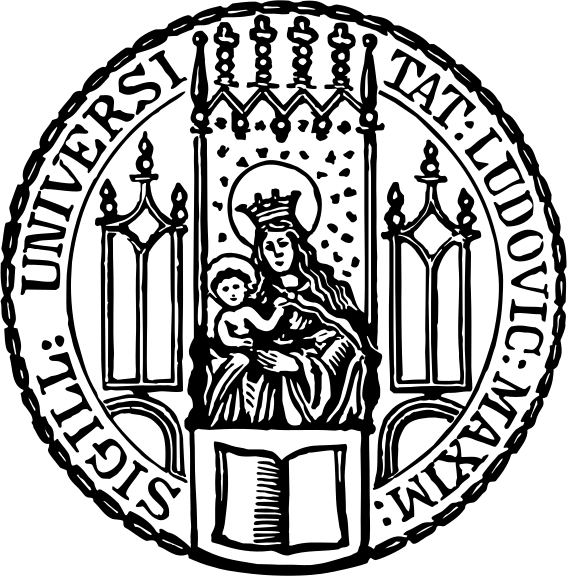
\includegraphics[width=.5\pagewidth]{\mediadir{image/emblem.pdf}}

    \usekomafont{subtitle}
    \@subtitle

    \vspace{.8em}
    \usekomafont{author}
    \@author

    \usekomafont{date}
    \@date

    \vspace{.8em}
    \usekomafont{publishers}
    \@publishers
  \end{center}
\end{titlepage}
\makeatother

\makeatletter
\begin{titlepage}
  \begin{otherlanguage}{ngerman}
    \begin{center}
      \usekomafont{subject}
      Mehrteilchen Quantenoptik

      \vspace{.8em}
      \usekomafont{title}\huge
      Hochpräzise zeitgemittelte optische Potentiale für ultrakalte Atome

      \vspace{.5em}
      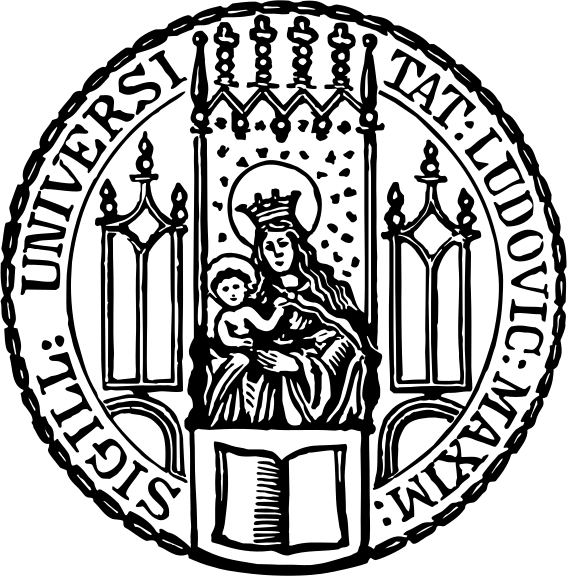
\includegraphics[width=.5\pagewidth]{\mediadir{image/emblem.pdf}}

      \usekomafont{subtitle}
      Bachelorarbeit von

      \vspace{.8em}
      \usekomafont{author}
      \@author

      \usekomafont{date}
      \@date

      \vspace{.8em}
      \usekomafont{publishers}
      entstanden unter der Betreuung von Prof. Dr. Immanuel Block,\\
      Dr. Monika Aidelsburger und Christian Schweitzer.
    \end{center}
  \end{otherlanguage}
\end{titlepage}
\makeatother

\addchap{Acknowledgement}

The success and final outcome of the present work required a lot of guidance
and assistance from many people. Without them it would not have been possible
for me to deliver this work and remember the exciting time I had in the past
weeks.

At most I want to thank my parents for their support, that I have been
privileged to benefit from all the years. Though my life involved many
unexpected turnarounds, I never felt left alone and could rely on your
diverse experience whenever the situation required it.

Further I want to thank Prof. Immanuel Bloch and Dr. Monika Aidelsburger for
creating and sustaining a fertile scientific environment. It has been a
refreshing novelty for me to have the opportunity to have inspiring
discussions at almost any time and to seamlessly implement new ideas without
being limited by the present material.

Equally I want to express my gratitude to all personal involved in the
formation process of my thesis. Especially I want to name Christian Schweizer
with whom it had been a great pleasure to work with. Further I want to thank
Till Klostermann for instantly sharing his deep insights in many problems I
have encountered and his help with the optical setup. Hendrik von Raven I want
to thank for his overall guidance with regard to the electronic equipment.
In addition I owe special thanks to Michael Schreiber who helped me understand
the theoretical foundations of atoms in optical lattices, David Wei for his
hospitality and productive discussions about the acousto-optic deflectors,
and of course biggest thanks to Bodo Hecker for his advice as electrical
engineer and distinct perspective on undergone challenges.

Finally I want to express my gratitude to my friend Dr. Abdullah Sarani for
his suggestions and advice on the final draft.

\addchap{Declearation of Authorship}

\addsec{Statutory Declearation}

I hereby declare that this thesis has been composed solely by myself except
where indicated otherwise by reference or acknowledgment.

The work presented has not been submitted, in whole or in part, in any
previous application for a degree.

\vspace{1em}
\textbf{Munich, \today}

\begin{abstract}
Ultracold atoms in optical lattices open up a wide range of possibilities
to simulate many-body quantum phenomena, which would elsewise be neither
computationally nor experimentally tangible.

The topology of the optical lattice is a decisive property of these kind
of experiments and therefore of major interest. Recently, efforts have been
reported to create novel optical potentials through the use of digital
micromirror arrays that permit alterations of localized potentials. Though
promising results have been achieved --- in particular for static potentials
--- limitations due to the mechanical nature of these mirror arrays arise,
for instance, with regard to dynamical control.

In the present work we present an alternative implementation of localized
optical lattice potentials based on acousto-optic deflectors and
direct digital synthesizers.

We will give a brief theoretical introduction into the main concepts, i.e.\
the interaction of neutral atoms with optical potentials as well as the
general operation of direct digital synthesizer and acousto-optic deflectors.
From the physics we can derive the requirements imposed on the technical
implementation of the \gls{rf} signal source and the deflection.

We will find that even though the platform of digital signal synthesis
generally suites our application in terms of modulation capabilities and
resolution, the particular implementation of the \gls{ad9910} demonstrates
several shortcomings.

In the second part we characterize the deflection efficiency of the
acousto-optic deflectors. Towards the end we try to minimize the variance of
the deflection efficiency by performing a random search on the amplitude
segments of the \gls{rf} signal. It turns out that the deflection efficiency
is a highly non-linear function of the applied \gls{rf} power and frequency.
Furthermore minimization of the deflection efficiency variances proves to be
very unstable. Though we can largely preclude electronic defects to be the
source of this behaviour, further investigation is required.
\end{abstract}


\tableofcontents

\chapter{Introduction}

Many quantum systems studied in condensed matter physics are experimentally
challenging to access as any interactions can destroy the carefully prepared
quantum states. As way forward, experiments with ultracold atoms in
optical lattices give us a highly contorllable environment, giving us the
opportunity to simulate and explore quantum effects and expand our current
understanding of quantum mechanics and statistical physics \cite{Gross2017}.

The central idea behind these types of experiments is to cool down neutral
atoms to micro Kelvin and below, and load them into an optical lattice. At
these temperatures atoms demonstrate quantum behaviour. The optical lattices
act as periodic potentials analogue to the periodic potential found inside
solid state crystal lattices \cite{Lewenstein2007}. Unlike to i.e. real solids
where we have limited prospects to amend a systems properties, lasers driven
by state of the art optics and electronics give us a wide range of well
controllable parameters.

\begin{figure}[h]
  \centering
  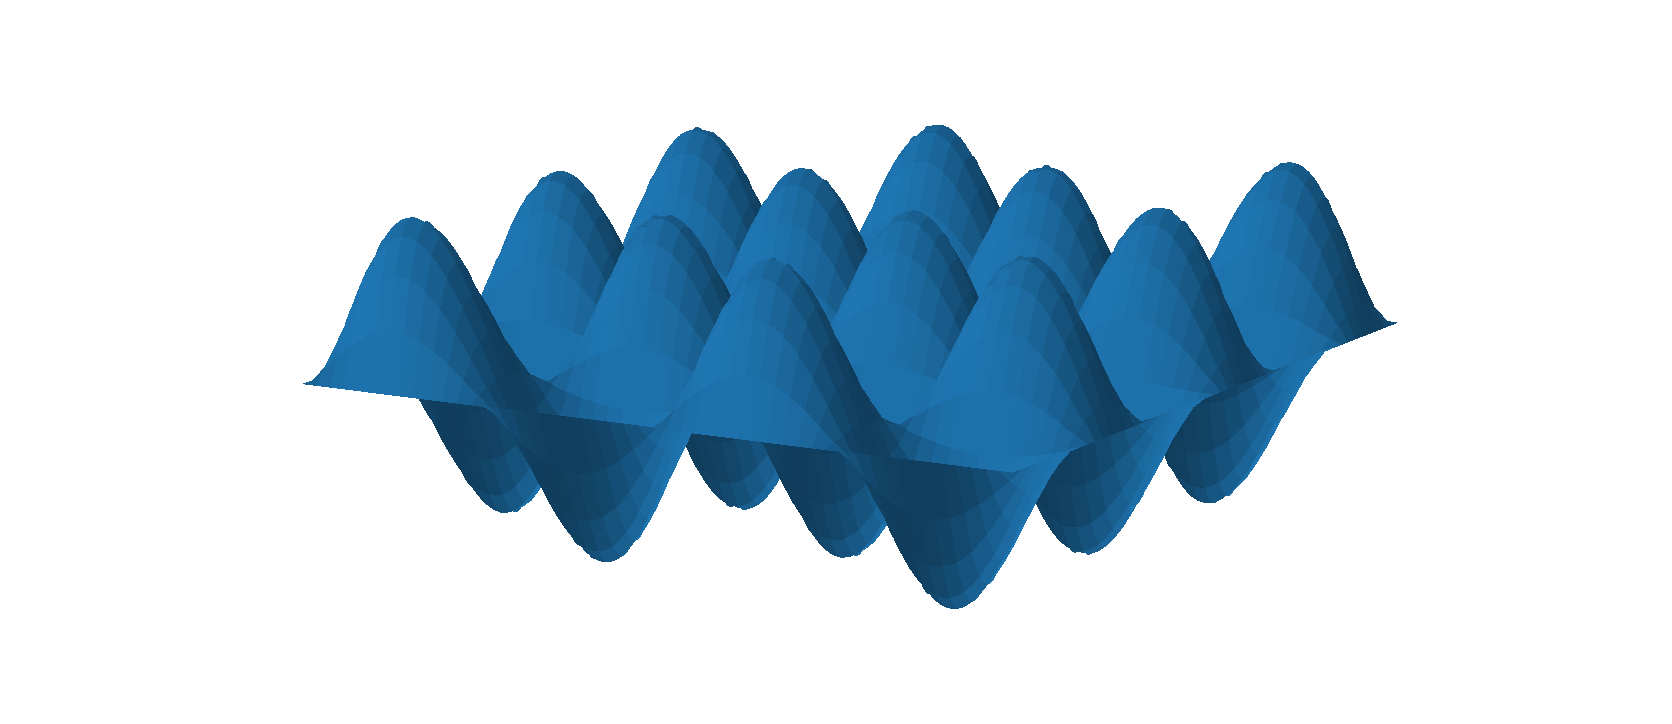
\includegraphics[width=.8\textwidth]{images/optlat/default.pdf}
  \captionsetup{width=.8\textwidth}
  \caption{Periodic potential of a 2D optical lattice. If the kinetic energy
  of the atoms is below the potential energy of the lattice, the atoms will
  locate around the potential minimas.}
  \label{fig:optlat}
\end{figure}

One of the parameters of interest is the ability to apply local potentials
to the system, that can be used to, among others, study lattice inpurities
or quantum interactions. In this work we will present and characterize one
possible implementation of such a local potential generating apparatus.

\section{Related Work}

Local manipulations of atoms inside optical lattices have been known for some
time in the embodiment of optical tweezers that allow trapping, stacking and
sorting of particles \cite{Tadmor2004}. Yet, only recently attempts to
interact with local particle clusters through high-precision time-averaged
optical potentials have been reported \cite{Roy2016}.

In the following we continue on the laid out work \cite{Hertlein2017} which
provided us with an optical setup for single-site manipulation using
\gls{aod} as well as considerations with regard to aperture limited
gaussian beam propagation.

\chapter{Hopping in optical lattices}

In the introduction we presented the concept of our envisaged potential
creation. In the following chapter we want to recapitulate the theoretical
foundations of optical lattices and quantum states theoreof. Finally we want
to derive an expression for the quantum tunnelling frequency in order to
estimate the time magnitude in which our apparatus has to operate.

\section{Atom-light interaction}

At first we need to ask ourselves how the laser field propagates as
perturbation potential to the Hamiltonian of the atomic system and how we can
express said potential by physical quantities we control in the experiment.

\subsection{Hamiltonian and dipole approximation}

The Hamiltonian of an electron in an external electromagnetic field reads
\begin{equation}
  \hat{H}_\text{em}
  =\frac{1}{2m}\left(\hat{\vb{p}}+e\vb{A}\right)^2-e\Phi+\hat{V}_0
  \label{eq:hamiltonian_em}
\end{equation}
with vector $\vb{A}$ and scalar potential $\Phi$ of the external field and
the Coulomb potential of the nucleus $\hat{V}_0$. \Cref{eq:hamiltonian_em} is
exact for the hydrogen atom and approximate for alkali atoms with one outer
electron.

Gauge freedom of the vector and scalar potential permits transformations of
type
\begin{align}
  \vb{A}\to\vb{A}+\grad{\chi}
  &&
  \Phi\to\Phi-\pdv{\chi}{t}
\end{align}
with gauge function $\chi(\vb{x},t)$. In the following we choose the gauge
function $\chi=-\vb{A}\cdot\vb{x}$ and assume the dipole approximation
$\vb{A}(\vb{x},t)\approx\vb{A}(t)$. The dipole approximation is reasonable as
wave length of visible light are much larger then atomic length scales
\cite{Gerry2004}. In the dipole approximation $\chi$ satisfies the Coulomb
gauge condition $\divergence{\vb{A}}=0$ allowing us to set $\Phi=0$ as no
external sources are present \cite{Jackson2005}. Finally we can rewrite
\cref{eq:hamiltonian_em} as
\begin{equation}
  \hat{H}_\text{dip}
  =\frac{\hat{\vb{p}}^2}{2m}+\hat{V}_0-\hat{\vb{d}}\cdot\vb{E}
  =\hat{H}_0+\hat{V}_\text{dip}
  \label{eq:hamiltonian_dip}
\end{equation}
with the dipole operator $\hat{\vb{d}}=-e\vb{x}$ and spatially homogeneous
light field $\vb{E}(t)$.

\subsection{Electrical field of an 1D optical lattice}

An one dimensional optical lattices can be generated through the interference
of two counter-propagating Gaussian beams, creating a standing wave
interference pattern. The electrical field component in such a case is given
by
\begin{equation}
  \vb{E}(t)
  =\vb{E}_0\cos(kz)\cos(\omega t)\exp(-\frac{2r^2}{w(z)^2})
  \label{eq:1d_lattice_efield_exact},
\end{equation}
wherein $r$ denotes the beam radius, $w(z)$ the spot size parameter and $k$
the angular wavenumber of the laser. The wavenumber relates to the laser
wavelength via $k=2\pi/\lambda$. The magnetic field component is chosen
in such a way that it satisfies the Maxwell equations but will not be
considered relevant any further as the electron only has a small magnetic
dipole. Analogue to \cite{Rom2009} we will now assume $w(z)\gg r$ and drop
the exponential term in \cref{eq:1d_lattice_efield_exact}, thus simplifying
\cref{eq:1d_lattice_efield_exact} to
\begin{equation}
  \vb{E}(t)
  \approx\vb{E}_0\cos(kz)\cos(\omega t)
  \label{eq:1d_lattice_efield_approx}.
\end{equation}
Note that even the electric field in \cref{eq:1d_lattice_efield_approx} has
a spatial dependency, the dipole approximation still holds in the atomic
reference frame.

\subsection{Effective dipole potential}

We are now going to solve \cref{eq:hamiltonian_dip} for the case of an
electric field of the form \cref{eq:1d_lattice_efield_approx} with
for-off-resonant laser wavelength $\lambda$ and finally derive an expression
for the effective dipole potential.

At $t<0$ the system is in the energy eigenstate $\ket{n}$ of the unperturbated
Hamiltonian
\begin{equation}
  \hat{H}_0\ket{n}
  =E_n\ket{n}
  =\hbar\omega_n\ket{n}
  \label{eq:eigenvalue_energy_unperturbated}.
\end{equation}
At $t>0$ the external light field appears instantaneous. The new state
$\ket{\psi}$ can be expanded in the complete base of the previous energy
eigenstates
\begin{equation}
  \ket{\psi}
  =\sum_nc_n(t)e^{-i\omega_nt}\ket{n}
  \label{eq:state_expansion_unperturbated}.
\end{equation}
Inserting \cref{eq:state_expansion_unperturbated} into the time-dependent
Schrödinger equation with dipole Hamiltonian \cref{eq:hamiltonian_dip} and
applying $\bra{m}e^{i\omega_mt}$ to the right hand side leads us to a set
of differential equations
\begin{equation}
  \dot{c}_m
  =-\frac{i}{\hbar}\sum_nc_n(t)e^{-i\omega_{nm}t}\bra{m}\hat{V}_\text{dip}\ket{n}
  \label{eq:differential_equation_population_dynamics}
\end{equation}
with $\omega_{nm}=\omega_n-\omega_m$, that describe the dynamics of the
probablity amplitudes $c_n(t)$. By using the electric field we derived in
\cref{eq:1d_lattice_efield_approx} we can rewrite the dipole transition
matrix elements
\begin{equation}
  \bra{m}\hat{V}_\text{dip}\ket{n}
  =\hbar\Omega_{nm}\cos(kz)\cos(\omega t)
  \label{eq:elements_dipole_transition_matrix}
\end{equation}
where we introduced the Rabi frequency
$\Omega_{nm}=\bra{n}\hat{\vb{d}}\cdot\vb{E}_0\ket{m}/\hbar$. Explicit values
for general dipole transition elements for one and two electron systems can
be found in \cite{Bethe1957}. Als the transition elements vanishes for states
with same parity, in particular do we have $\Omega_{nn}=0$
\cite{Bartelmann2018}.

From now on we assume a two state system that initially is only populated in
the ground state $c_g(0)=1,c_e(0)=0$ and the dynamics in
\cref{eq:differential_equation_population_dynamics} are simply described by
\begin{align}
  i\dot{c}_g=\Omega_0c_e(t)\cos(kz)\cos(\omega t)e^{+i\omega_0 t} &&
  i\dot{c}_e=\Omega_0c_g(t)\cos(kz)\cos(\omega t)e^{-i\omega_0 t}
  \label{eq:differential_equation_population_dynamics_two_state_system}.
\end{align}
Expansion of $\cos(\omega t)$ in terms of the exponential function and
dropping $e^{\pm i(\omega+\omega_0)t}$ yields
\begin{align}
  i\dot{c}_g\approx\frac{\Omega_0}{2}c_e(t)\cos(kz)e^{+i\Delta\omega t} &&
  i\dot{c}_e\approx\frac{\Omega_0}{2}c_g(t)\cos(kz)e^{-i\Delta\omega t}
  \label{eq:differential_equation_population_dynamics_two_state_system_rwa}.
\end{align}
The so-called rotating wave approximation is motivated by the fact that
oscillations of frequency $\omega+\omega_0$ are fast compared to changes in
the population dynamics and therefore vanish on average.

We now define $a_g=c_g$ and $a_e=c_ee^{i\Delta\omega t}$ and refine
\cref{eq:differential_equation_population_dynamics_two_state_system_rwa} by
\begin{align}
  i\dot{a}_g=\frac{\Omega_0}{2}a_e(t)\cos(kz) &&
  i\dot{a}_e=\frac{\Omega_0}{2}a_g(t)\cos(kz)-a_e\Delta\omega
  \label{eq:differential_equation_population_dynamics_two_state_system_shift}.
\end{align}
In the former form we can diagonalize the Hamiltonian and find energy
eigenvalues to be
\begin{equation}
  E_{e,g}
  =\frac{\hbar}{2}\left(-\Delta\omega\mp\sqrt{\Omega_0^2+\Delta\omega^2}\right)
  \approx
  =\mp\frac{\hbar\Omega_0^2}{4\Delta\omega}
  \label{eq:eigenvalues_energy_light_shift}
\end{equation}
where we applied Taylor expansion to the square root for
$\Delta\omega\gg\Omega_0$.

In summary atoms in an external off-resonant light field with experience an
effective periodic dipole potential
\begin{equation}
  \hat{V}_\text{eff}
  =V_0\cos^2(kz)
  \qc
  V_0
  =\frac{\hbar\Omega}{4\Delta\omega}\cos^2(kz)
  =\frac{\hbar I_0\cos^2(kz)}{2c_0\epsilon_0\Delta\omega}
  \label{eq:potential_effective}
\end{equation}
with vacuum speed of light $c_0$, dielectric constant $\epsilon_0$ and
maximum intensity $I_0$. Same results can also be obtained by the use of
second order perturbation theory, however the presented approach is more
clear on assumptions and time dependence \cite{Grimm2008}.

\section{Harmonic approximation}

Given the effective lattice potential \cref{eq:potential_effective} the
effective lattice Hamiltonian reads
\begin{equation}
  \hat{H}_\text{eff}
  =\frac{\hat{p}^2}{2m}+\hat{V}_\text{eff}
  \label{eq:hamiltonian_effective}.
\end{equation}
One first naive approach to solve the time-independent Schrödinger equation
subject to the effective lattice Hamiltonian would be to Taylor expand
the effective potential in second order
\begin{equation}
  \hat{V}_\text{eff}
  =V_0\cos^2(kx)
  \approx V_0\left(1-(kx)^2\right)
  \label{eq:potential_harmonic_approximation}
\end{equation}
and give us the Hamiltonian of a linear harmonic quantum oscillator
\begin{equation}
\begin{equation}
  \hat{H}_\text{har}-V_0
  =\frac{\hat{p}^2}{2m}-V_0k^2x^2
  \label{eq:hamiltonian_harmonic_approximation}
\end{equation}
with well-known energy levels $E_n=\hbar\omega(2n+1)/2$ and frequency
$\omega=\sqrt{V_0/m}k=\sqrt{2V_0E_r}/\hbar$, where we defined the recoil
energy $E_r=(\hbar k)^2/(2m)$ as an atom-independent energy scale.

The harmonic approximation is valid for very deep potentials $V_0\gg E$.
Unfortunately the Gaussian wave functions of the harmonic oscillator decay
fast at the potential boundary such that we have vanishing probability to
find a particle tunneling through the potential.

\section{Periodic lattice potentials}

The following section is dedicated to the quantum mechanics of periodic
lattice potentials. After we revise the formulation of lattice structures,
we will examine Bloch and Wannier states as well as the energy bands arising
in periodic lattice potentials.

\subsection{Lattice structures}

A Bravais lattice of dimension $N$ consists of the discrete points
\begin{equation}
  \vb{r}
  =\bra{\vb{x}}\ket{\vb{r}}
  =\sum_{i=1}^Nn_i\vb{a}_i
  \qc n_1,\dots,n_N\in\mathbb{Z}
\end{equation}
where $\vb{a}_i$ are the primitive vectors that span the primitive lattice
cell.

We define the reciprocal lattice as the discrete points
\begin{equation}
  \vb{g}
  =\bra{\vb{p}}\ket{\vb{g}}
  =\sum_{i=1}^Nm_i\vb{b}_i
  \qc m_1,\dots,m_N\in\mathbb{Z}
\end{equation}
that satisfy the condition $\exp(\vb{r}\cdot\vb{g})=1$. For a simple cubic
lattice structure $\vb{b}_i=2\pi\vb{a}/{{\vb{a}_i}^2}$ satisfies said
condition. For the subsequent sections we will only consider the one
dimensional simple cubic lattice. Cubic lattices of higher dimension however
can be easily obtained by superposition of the potentials.

As the reciprocal lattice space can be seen as the Fourier transform of the
Bravais lattice, it is especially simple to express periodic functions and it
suggests the representation of periodic potentials in reciprocal lattice
space. Let $\ket{g_n}$ denote the $n$th reciprocal lattice point then the
transformation rule is
\begin{equation}
  \bra{g_n}\hat{V}\ket{g_m}
  =\int\dd{x}\bra{g_n}\ket{x}^*V(x)\bra{g_m}\ket{x}
  =\int\dd{x}V(x)e^{2ikx(n-m)}
  \label{eq:potential_in_reciprocal_lattice}.
\end{equation}
Evaluation of \cref{eq:potential_in_reciprocal_lattice} for a specific
potential will usually yield a finite number of terms in dependence of
$n-m$ as we actually determine the Fourier coefficients of a discrete Fourier
transform.

\subsection{Bloch states}

Bloch's theorem states that for a periodic lattice potential
\begin{equation}
  V_\text{lat}(\vb{x}+\vb{a})=V_\text{lat}(\vb{x})
  \label{eq:potential_periodic}
\end{equation}
there exists a complete set of wavefunctions that are energy eigenstates
of the Hamiltonian
\begin{equation}
  \hat{H}_\text{lat}
  =\frac{\hat{\vb{p}}^2}{2m}+\hat{V}_\text{lat}
  \label{eq:hamiltonian_periodic},
\end{equation}
and each of these Bloch waves can be written into the form
\begin{equation}
  \bra{\vb{x}}\ket{\Psi^n_{\vb{q}}}
  =\Psi^n_{\vb{q}}(\vb{x})
  =e^{i\vb{q}\cdot\vb{x}}\psi^n_{\vb{q}}(\vb{x})
  \label{eq:state_bloch}
\end{equation}
with $\psi^n_{\vb{q}}(\vb{x}+\vb{a})=\psi^n_{\vb{q}}(\vb{x})$, wave vector
$\vb{q}$ and bandindex $n$. We confine the wave number to the first Brillouin
zone $-k<q<+k$. For a proof of Bloch's theorem see \cite{Roessler2004} or
\cite{Bartelmann2018}.

\subsection{Energy band structure}

The Bloch states \cref{eq:state_bloch} can be used as ansatz to solve the
periodic lattice Hamiltonian
\begin{equation}
  \hat{H}_\text{lat}
  =\frac{\hat{p}^2}{2m}+\hat{V}_\text{lat}
  \label{eq:hamiltonian_lattice}.
\end{equation}
We notice that by the product rule
$\hat{p}^2\Psi^n_q(x)=e^{iqx}(\hat{p}+\hbar q)\psi^n_q(x)$,
thus we find
\begin{equation}
  E^n_q\ket{\Psi^n_{q}}
  =\hat{H}_{lat}\ket{\Psi^n_{q}}
  =e^{iqx}\left(\frac{(\hat{p}+\hbar q)^2}{2m}+\hat{V}_\text{lat}\right)\ket{\psi^n_{q}}
  \label{eq:eigenvalue_energy_lattice}.
\end{equation}
Expansion of the state $\ket{n,q}$ in states of the reciprocal lattice returns
\begin{equation}
  \ket{\Psi^n_q}
  =\left(\sum_s\ket{g_s}\bra{g_s}\right)\ket{\Psi^n_q}
  =\sum_s\braket{g_s}{\Psi^n_q}\ket{g_s}
  =\sum_sc^n_{sq}\ket{g_s}
  \label{eq:state_bloch_in_reciprocal_lattice}.
\end{equation}
The momentum eigenvalues of the state $\ket{g_s}$ can be found by expansion
into position space
\begin{equation}
  \hat{p}\ket{g_s}
  =\int\int\dd{x}\dd{y}\ket{y}\bra{y}\hat{p}\ket{x}\bra{x}\ket{g_s}
  \label{eq:eigenvalue_momentum_reciprocal_lattice1}.
\end{equation}
With $\bra{y}\hat{p}\ket{x}=-i\hbar\delta(y-x)\dv{x}$ we can take the
derivative of $\bra{x}\ket{g_s}=e^{2ikxs}$ and simplify
\cref{eq:eigenvalue_momentum_reciprocal_lattice1} down to
\begin{equation}
  \hat{p}\ket{g_s}
  =2\hbar ks\int\dd{x}\ket{x}\bra{x}\ket{g_s}
  =2\hbar ks\ket{g_s}
  \label{eq:eigenvalue_momentum_reciprocal_lattice2}.
\end{equation}
Finally we insert \cref{eq:state_bloch_in_reciprocal_lattice} into
\cref{eq:eigenvalue_energy_lattice} and apply $\bra{g_t}$ to the
right hand side while using \cref{eq:potential_in_reciprocal_lattice} and
\cref{eq:eigenvalue_momentum_reciprocal_lattice2}, yielding
\begin{equation}
  E^n_qc^n_{tq}
  =c^n_{tq}\frac{(2s+q/k)^2}{2m}E_r+\sum_sc^n_{sq}\bra{g_t}\hat{V}_\text{lat}\ket{g_s}
  \label{eq:eigenvalue_energy_lattice_explicit}
\end{equation}
with recoil energy $E_r=\hbar^2k^2/(2m)$.
\Cref{eq:eigenvalue_energy_lattice_explicit} has to be solved for known
$\hat{V}_\text{lat}$ numerically. We will do this later for the effective
optical lattice potential from \cref{eq:potential_effective}.

\subsection{Wannier states}

So far we studied the effects of a periodic lattice potential on the energy
levels and the Bloch wave functions that propagate over the complete lattice.
Lattice hopping however is a local effect, therefore we need a spatially
localized set of wave functions to describe the effect of lattice hopping.
Fortunately the so called Wannier fullfill these requirements.

The orthodox definition of the Wannier function with bandindex $n$ at lattice
site $l$ reads
\begin{equation}
  \ket{\phi^n_{l}}
  =\frac{1}{\sqrt{N}}\sum_qe^{-iqla}\ket{\Psi^n_{q}}
  \label{eq:state_wannier_orthodox}
\end{equation}
wherein $\ket{\Psi^n_q}$ is the Bloch wave functions from
\cref{eq:state_bloch}, $N$ the total number of lattice sites and the sum
over $q$ is confined to the first Brillouin zone with $q$ that satisfy the
periodic boundary condition $q=2ks/N$ with integer $s\in\mathbb{Z}$.

\section{Hopping frequency}

Quantum mechanics predicts a nonzero probability for particles to tunnel
through an energy barrier. Lattice hopping describes this phenomena of atoms
tunneling through the optical lattice potentials to other lattice sites. In
this section we want to find an expression for the probability amplitude of
such hopping effects.



\chapter{Digital signal synthesis}

The previous chapters have covered the physical theory behind our targeted
application. From that we were able to recover some technical requirements
imposed on our implementation. In this chapter we will review the fundamentals
of digital signal synthesis as \gls{rf} signal source to control the \gls{aod}.

\gls{dds} offer some distinct advantages over traditional analog synthesiser.
For one they can cover up a wide frequency range with high tuning resolution.
In contrast thereto analog devices have to be fitted to a narrow operation
range and are subject to variations caused by aging, thermal drift and
manufacturing. In addition \gls{dds} permit extremly fast, phase-continous
changes of the output signal parameters, without the loop-settling behaviour
known to analog devices. Most recently \gls{dds} can easily be integrated into
existing digital circuits giving rise to a cost-competitive remote
controllable device. Overall these advantages make the \gls{dds} an attractive
solution for our projected application \gls{rf} signal source \cite{ADTutDDS}.

\section{Operating principle}

\Cref{fig:dds_simple_architecture} depicts a flow diagram of the components
that make up a simple \gls{dds}. Given a system clock frequency $f_\text{sys}$
and the desired output frequency $f_\text{out}$ one can derive the phase
accumulator increment
\begin{equation}
  \Delta\varphi
  =
  \lceil\frac{f_\text{out}}{f_\text{sys}}2^N+\frac{1}{2}\rceil
  \label{eq:dds_phase_increment}
\end{equation}
where $N$ denotes the number of bits the phase accumulator can store.
\begin{figure}[ht]
  \centering
  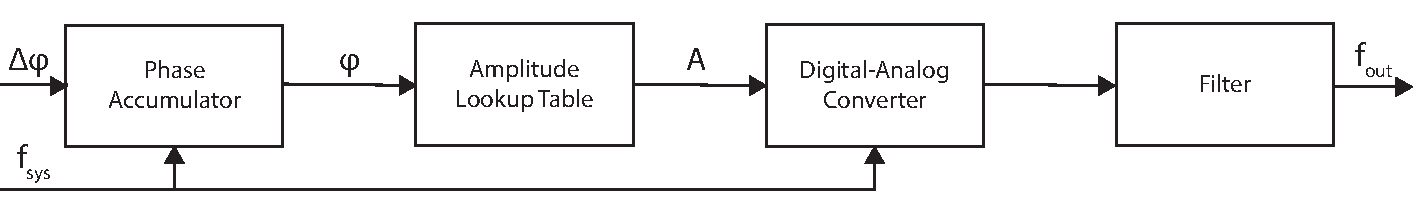
\includegraphics[width=\textwidth]{\figuredir{digital-signal-synthesis/simple-architecture.pdf}}
  \captionsetup{width=.8\textwidth}
  \caption{Signal flow through a simple \gls{dds}. The output frequency
    determines a phase step by which the accumulator is incremented at each
    clock cycle. The value of the phase accumulator is used for amplitude
    lookup of the desired output signal shape. A \gls{dac} outputs the signal
    which then is filtered to smooth the discrete \gls{dac} output.
  }\label{fig:dds_simple_architecture}
\end{figure}
For every clock cycle the phase accumulator is incremented by $\Delta\varphi$.
On overflow of the accumulator a new signal period starts. The phase
accumulator value is used to lookup the corresponding amplitude value of the
desired output signal shape. For example one can use a lookup table with the
values of a sinusoidal output signal. Alternatively one can omit the lookup
table and output a sawtooth output signal by suppling the phase accumulator
output directly to the \gls{dac} or a square wave signal output by suppling
the most significant bit directly. Finally a \gls{dac} converts the digital
amplitude value to an analog signal. An optional analog filter can be used to
smooth the discrete output. In \Cref{fig:dds_simple_output} the signal at the
different processing stages inside a simple \gls{dds} are presented for a
\SI{8}{\bit} precision, system clock frequency
$f_\text{sys}=\SI{1}{\giga\hertz}$ and output frequency
$f_\text{out}=\SI{100}{\mega\hertz}$.
\begin{figure}[ht]
  \centering
  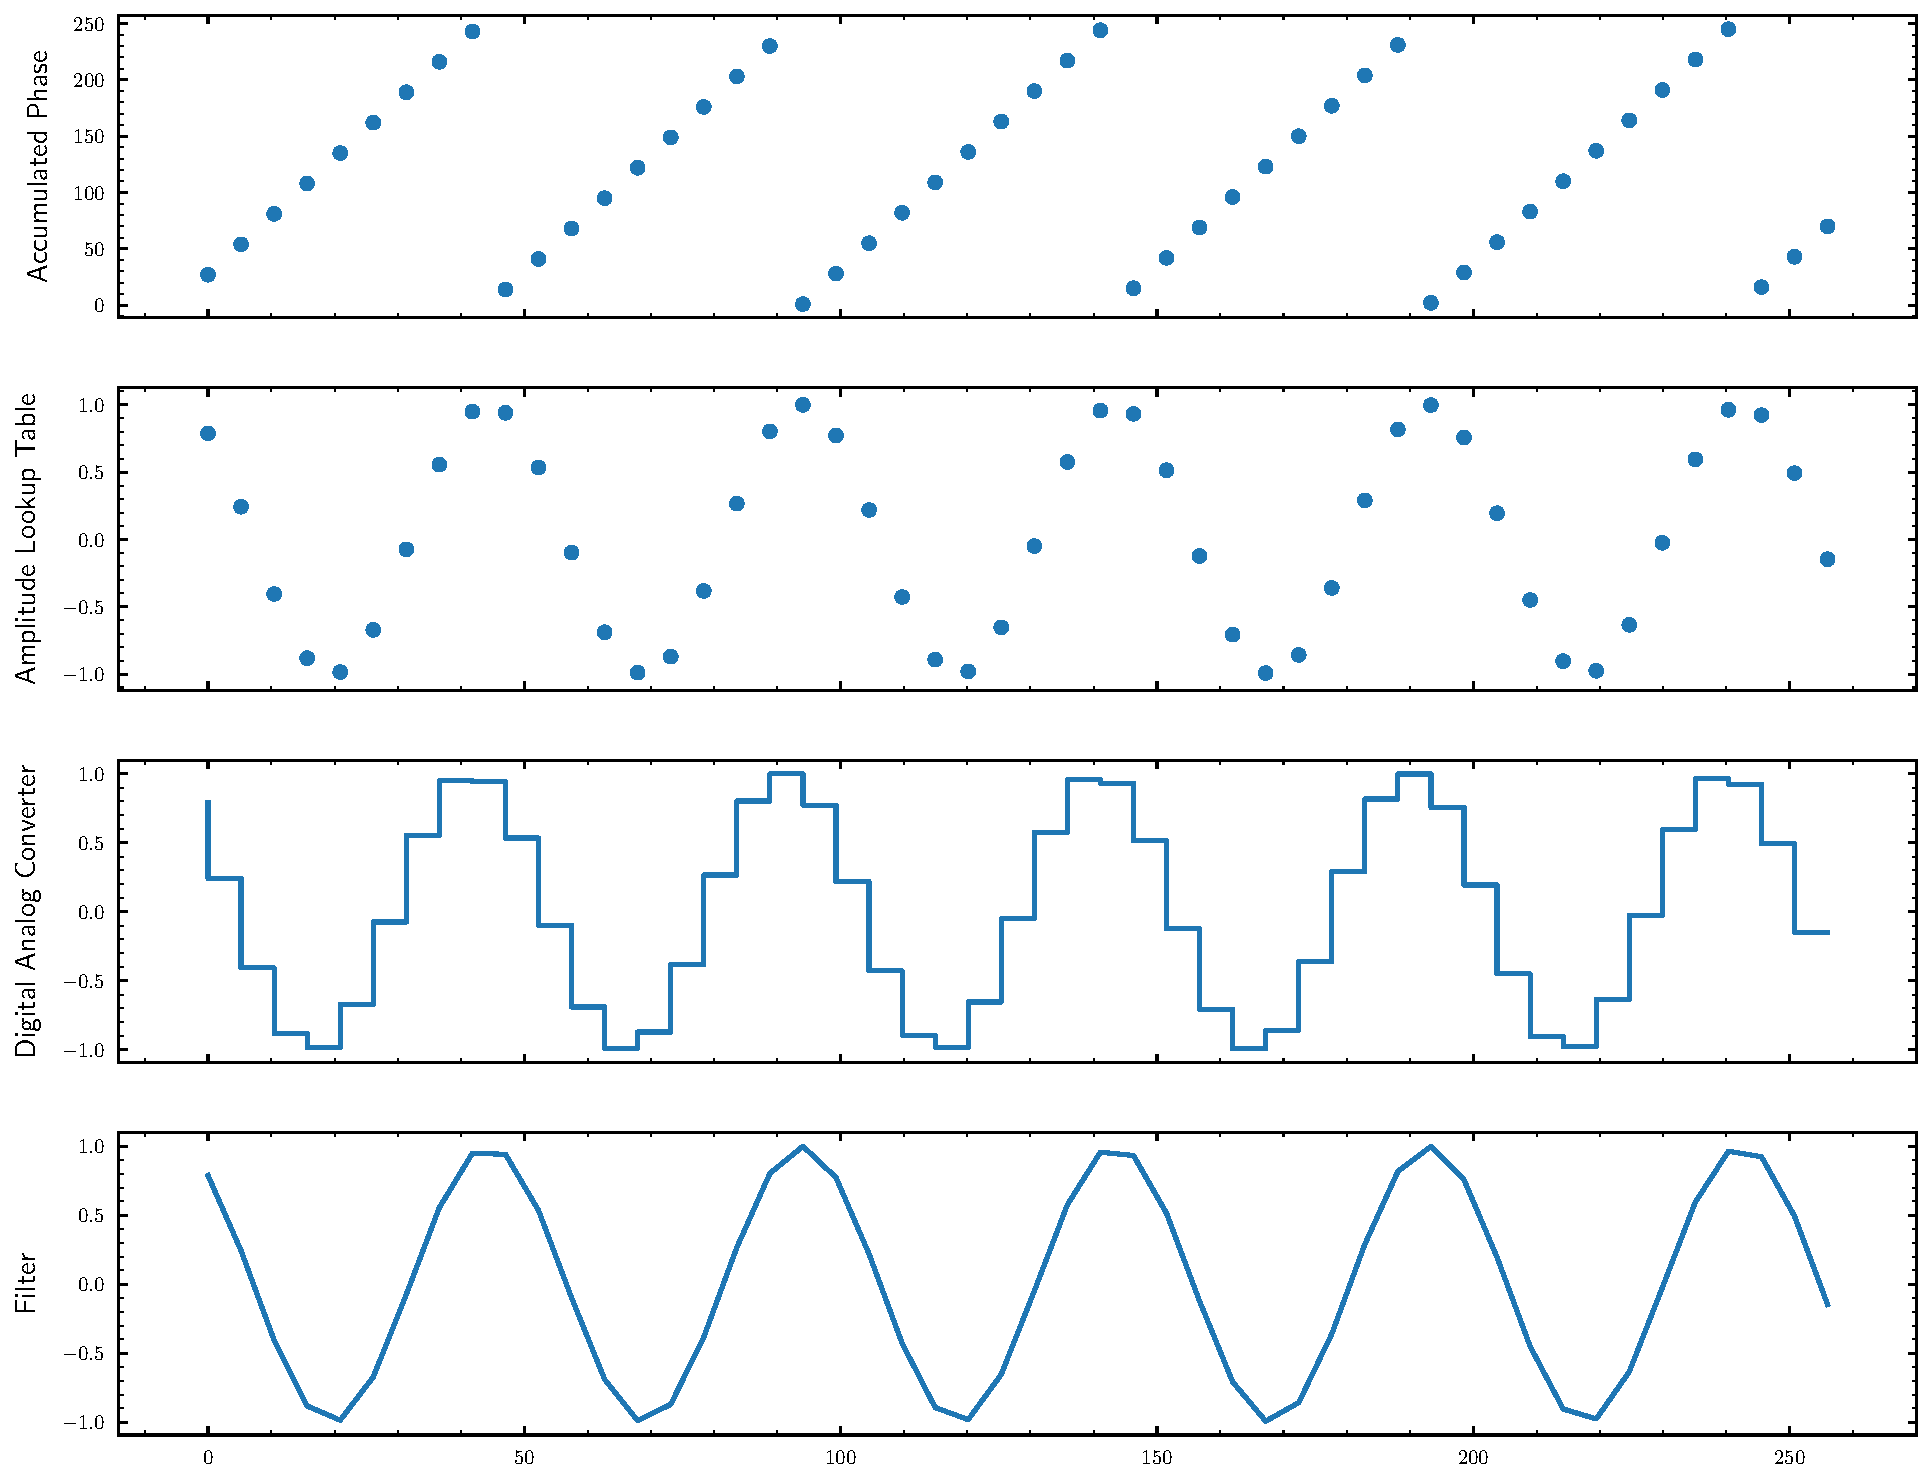
\includegraphics[width=\textwidth]{\figuredir{digital-signal-synthesis/simple-output.pdf}}
  \captionsetup{width=.8\textwidth}
  \caption{Signal outputs at different stages in a simple \gls{dds}. The
    phase accumulator is incremented at each clock cycle by $\Delta\phi$. The
    phase accumulator value is used to lookup a sinusoidal amplitude value
    that is supplied to a \gls{dac}. The final result is smoothed using a
    filter.}\label{fig:dds_simple_output}
\end{figure}
In the first column of \Cref{fig:dds_simple_output} we can see how the phase
accumulator is incremented on every clock iteration and resets on overflow.
In the second column the lookup table has been used to return the
corresponding cosine amplitude. We can see a difference in output shape
between even and odd samples. This is caused by the fact that the phase
increment is not a divisor of the phase accumulator size and we will later
discuss workarounds.

\subsection{Clock generation}

The Nyquist-Shannon sampling theorem states that for a given sample rate a
perfect reconstruction is guaranteed possible for
$f_\text{out}<f_\text{samp}/2$. Until now we have considered the system clock
frequency $f_\text{sys}=f_\text{samp}$ as given. In practice reliable
reference signals are clocked below the desired output range and thereby
cannot directly be used as system clock according to the Nyquist-Shannon
sampling theorem.
\begin{figure}[ht]
  \centering
  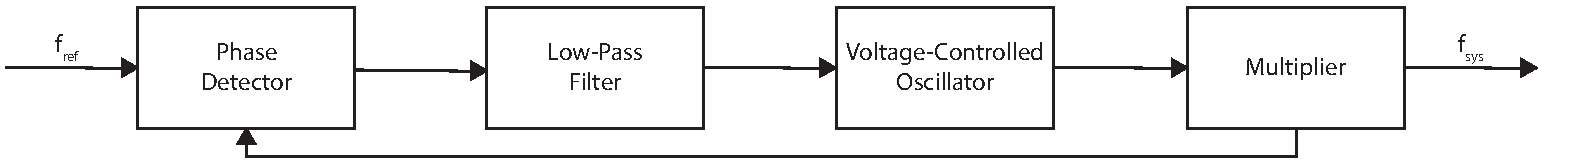
\includegraphics[width=\textwidth]{\figuredir{digital-signal-synthesis/clock-generation.pdf}}
  \captionsetup{width=.8\textwidth}
  \caption{Clock generation signal generation with \gls{pll} and multiplier.
    The phase detector compares the output system phase with the reference
    phase and yields a non-linear error response. The low-pass filter removes
    fast oscillations. The \gls{vco} changes the output phase in dependence
    of the error response. Finally system and reference phase will go in lock.
    }\label{fig:dds_clock_generation}
\end{figure}
\Cref{fig:dds_clock_generation} the system clock generation from a reference
signal is illustrated. The phase detector yields a non-linear error response
comparing the output signal phase with the reference signal phase. After a
low-pass filter removes fast oscillations a \gls{vco} changes its phase
proportional to the error signal. Finally a frequency multiplier creates
harmonics of the reference frequency and extracts a programmed frequency
multiple of $M$ such that the system frequency relates to the reference
clock by $f_\text{sys}=Mf_\text{ref}$ with $1<M\in\mathbb{N}$.

\subsection{Parameter modulation}

So far we only discussed the case of frequency modulation. We will see that
the previous architecture can be easily extended to support amplitude
and phase modulation too.
\begin{figure}[ht]
  \centering
  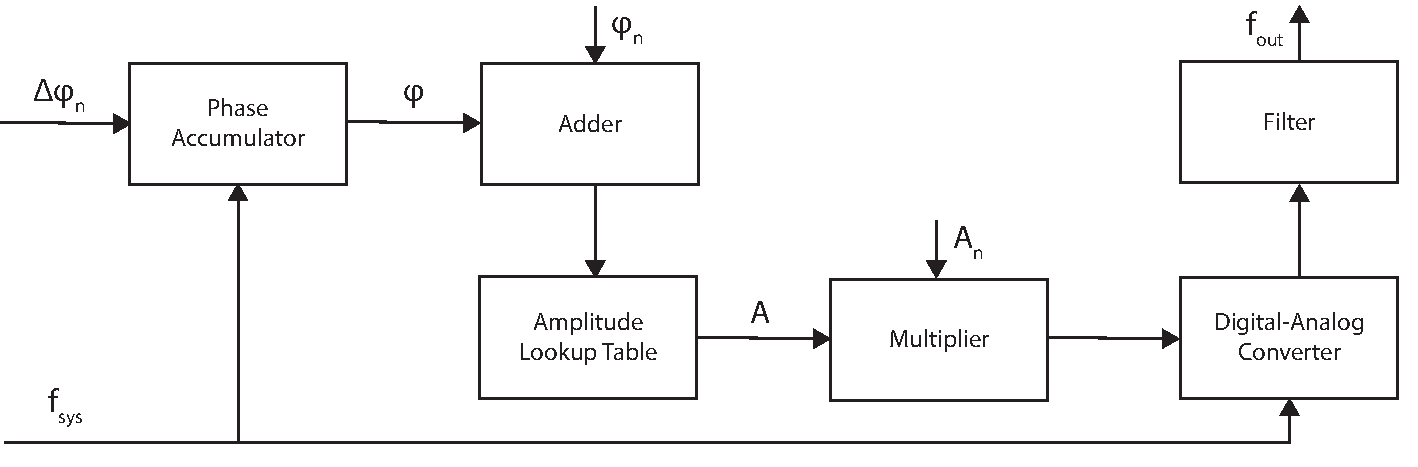
\includegraphics[width=\textwidth]{\figuredir{digital-signal-synthesis/modulation-architecture.pdf}}
  \captionsetup{width=.8\textwidth}
  \caption{
    \gls{dds} architecture supporting modulation of frequency, amplitude and
    phase offset parameters. Phase accumulator increment is now time dependent.
    The phase offset is also time dependent is added as last step to the
    phase accumulator before supplied to the \gls{dac}. The time dependent
    amplitude parameter is multiplied with the amplitude obtained from the
    lookup table.
    }\label{fig:dds_modulation_architecture}
\end{figure}
In \Cref{fig:dds_modulation_architecture} we can see one realization of an
architecture that supports amplitude, frequency and phase modulation. The main
components are the same as in \Cref{fig:dds_simple_architecture}. In addition
we have an adder for a time dependent phase offset and a multiplier for the
digital amplitude value obtained from the lookup table. The time dependence
of the parameters can be either determined by reading from memory or through
generation of another circuit. In a later section we will discuss the case of
a linear frequency sweep provided by a digital ramp.

\section{Quantization errors}
\section{Frequency response}

\section{Operating range}

We apply a reference signal of
\begin{equation}
  f_\text{ref}=\SI{10}{\mega\hertz}
\end{equation}
configured to be used with a \gls{pll} multiplier of
$N=100$ yielding a system clock of
\begin{equation}
  f_\text{sys}=Nf_\text{ref}=\SI{1}{\giga\hertz}.
\end{equation}
The timer clock used for the linear ramp and memory playback runs with
a quarter of the system clock
\begin{equation}
  f_\text{timer}=f_\text{sys}/4=\SI{250}{\mega\hertz}.
\end{equation}

The \gls{ad9910} uses a \SI{14}{\bit} \gls{asf} and \SI{32}{\bit} \gls{ftw}
to parameterize amplitude $A(t)$ and output frequency $f(t)$ by
\begin{align}
  FTW
  :=
  \left\lfloor2^{32}\left(\frac{f_\text{out}}{f_\text{sys}}\right)\right\rceil
  &&
  ASF
  :=
  \left\lfloor\frac{A_\text{out}}{2^{14}}\right\rceil
  \label{eq:elec:ftwasf}
\end{align}
wherein $\lfloor{\cdot}\rceil$ rounds the given float to the nearest integer.
The theoretical limit for the maximum output frequency then is found via
\begin{equation*}
  f_\text{max}
  =
  \left(1-\frac{2^{31}-1}{2^{32}}\right)f_\text{sys}
  =
  \left(\frac{1}{2}-\frac{1}{2^{31}}\right)f_\text{sys}
  \approx
  \frac{1}{2}f_\text{sys}
  =
  \SI{500}{\mega\hertz}.
\end{equation*}
Yet the datasheet \cite{AD9910} reports $f_\text{max}=\SI{420}{\mega\hertz}$
and in fact we found the output signal to be very noisy at the theoretical
limit.

We continue with the assessment of the digital ramp that does a unidrectional
linear sweep on the frequency from \SI{90}{\mega\hertz} to
\SI{110}{\mega\hertz}. The digital ramp of the \gls{ad9910} lets us define
a \gls{ftw} step $M$ word of \SI{32}{\bit} as well as a step rate word $S$ of
\SI{16}{\bit} resolution. They relate to the frequency step and the time
step through
\begin{align}
  \Delta f
  =
  \frac{M}{2^{32}}f_\text{sys}
  &&
  \Delta t
  =
  \frac{S}{f_\text{timer}}
  =
  \frac{S}{4f_\text{sys}}.
  \label{eq:elec:step}
\end{align}
The sweep duration is deterimened by $S,M$ through
\begin{equation}
  T_\text{duration}
  =
  \frac{f_\text{upper}-f_\text{lower}}{\Delta f}\Delta t
  =
  2^{32}\frac{f_\text{upper}-f_\text{lower}}{f_\text{sys}}\frac{S/M}{f_\text{timer}}
\end{equation}
for a target sweep duration of $T_\text{duration}=\SI{10}{ms}$ we find
\begin{equation*}
  \frac{S}{M}
  =
  \frac{T f_\text{timer}}{2^{32}}\frac{f_\text{sys}}{f_\text{upper}-f_\text{lower}}
  =
  \frac{10^9}{2^{35}}
  \approx
  \num{2.9104e-2}
  =
  \frac{1819}{62500}
\end{equation*}
the last step can be obtained by best ratio approximation using continued
fractions as for example described in \cite{Ashley2003}. It should be kept in
mind that the best ratio approximation is likable to introduce an error,
therefore realistic durations may differ from the configured value and it
is possible that better approximations exist that allow smaller $\Delta f,
\Delta t$, thus providing a sweep resolution. In the above case the given
time duration translates to
\begin{align*}
  \Delta f
  =
  \frac{62500}{2^{32}}f_\text{sys}
  \approx
  \SI{145}{\kilo\hertz}
  &&
  \Delta t
  =
  \frac{1819}{f_\text{timer}}
  \approx
  \SI{7.28}{\micro\second}
\end{align*}
or $(f_\text{upper}-f_\text{lower})/\Delta f=138$ discrete data points.

Eventually we are left with the assessment of the amplitude sequence. The
memory fits at most 1024 discrete amplitude values and the \gls{ad9910}
allows us to set the time spent at each amplitude value via the \SI{16}{\bit}
playback rate $P$ word
\begin{equation}
  \Delta t
  =
  \frac{P}{f_\text{timer}}
  =
  \frac{4P}{f_\text{sys}}
\end{equation}
which gives us range from $\min\Delta t=\SI{4}{\nano\second}$ to
$\max\Delta t=\SI{26.14}{\micro\second}$. As we incorporate all of the 1024
data points this gives us a duration range from about
$\min T=\SI{4}{\micro\second}$ to $\max T=\SI{26.84}{\milli\second}$.


\chapter{Experimental setup}

The exerimental setup was largely adopted from \cite{Hertlein2017}, amendments
made include the \gls{rf} signal source of the \gls{aod} and an additional
photodiode to measure the deflected beam intensity.

\section{Optics}

The optical setup can be dissect into a closed first section that reduces
the power of the $\SI{532}{\nano\meter}$ laser source from $\SI{10}{\watt}$
to below $\SI{2}{\milli\watt}$ and an open second section for beam deflection.
Both sections are connected through a \gls{smf}.

\subsection{Power reduction}
\label{sec:powerbox}

Because of safety concerns the power reduction section is confined into a
visually sealed superstructure. \Cref{fig:powerbox} reveals the inside of the
power reduction box.

\begin{figure}[h]
  \centering
  \includegraphics[width=\textwidth]{standalone/powerbox.pdf}
  \caption{Optical configuration of the power reduction section.}
  \label{fig:powerbox}
\end{figure}

The laser beam leaving the laser source is polarized by a $\lambda/2$ retarder
plate such that the succeeding high power beamsplitter BS can divert the
majority of the beams power into a high power beam dump.
Afterwards mirrors M1 and M2 direct the beam towards the center of a $2:1$
telescope composed of two lenses L1, L2 with focal lengths
$f_1=\SI{100}{\milli\meter}$ and $f_2=\SI{50}{\milli\meter}$.
An \gls{aom} diffracts the laser beam into multiple orders. Mirrors M3, M4
project theses orders onto a pinhole which is configured to intromit only the
the first order deflection. The intensity of the first order is subject to
amplitude modulation apllied to the \gls{aom}.
Finally a tunable $\lambda/2$ retarder plate can be used to couple the beam
polarization with the \gls{smf}.

\subsection{Beam deflection and detection}
\label{sec:deflection}

The section for beam deflection and detection as disclosed in
\cref{fig:deflection} receives the down-powered laser beam from previously
described section by a \gls{smf}. Hereinafter the beam passes a tunable
retarder plate and beam splitter BS1. The tunable retarder plate can be used
to adjust the beam intensity without having to access the power box.
A second polarizer with cube BS2 is used to branch off a part of the beam
to a photodiode PD1 that is positioned to be at the focal point of lens L1.
Photodiode PD1 is connected via a control system with the amplitude
modulation of the \gls{aom} depicted in \cref{fig:powerbox} to stabilize
the laser intensity against i.e. thermal drifts.

\begin{figure}[h]
  \centering
  \includegraphics[width=\textwidth]{standalone/deflection.pdf}
  \caption{Optical configuration of the beam deflection section.}
  \label{fig:deflection}
\end{figure}

For horizontal and vertical beam deflection two \gls{aod}s are used. A $1:1$
telescope comprised of two lenses L2, L3
each with focal length $f_2=f_3=\SI{250}{\milli\meter}$ projects the beam
on a pair of objectives that are built of lenses L4 to L7. The purpose of the
objective pair is to focus the laser on to the atom plane.
Consecutively the laser is reflected by a pair of mirrors M3 and M4 to the
part intended for detection. Lens L8 acts as a camera lens and projects the
beam to infinite focus on to the CCD camera sensor. Cube BS3 forks a portion
of the beam away from the CCD camera on to mirror M5 that guides the beam
towards lens L9 in order to focus the beam onto a second photodiode PD2.

\section{Electronics}

Beforehand we described the optical setups used. Now we want to emphasize
on the electronics how they are integrated into the optical setup.

\subsection{Signal source}

The requirements placed by the two \gls{aod} demand flexible but precise
\gls{rf} sources. Fortunately we can resort to a custom made signal
sources based on the \gls{ad9910} \gls{dds} \cite{AD9910} \gls{ic} that can
operate up to \SI{420}{\mega\hertz} and allows modulation of amplitude,
frequency and phase offset by either a constant value or through a single
digital ramp or playback from a memory sequence.

The signal output of the \gls{dds} is of the form
\begin{equation}
  U(t)=A(t)\sin(2\pi f(t)+\phi(t)).
  \label{eq:dds:signal}
\end{equation}
In the following we will ignore the unsynced phase offset, thus setting
$\phi=0$. In case of the single \gls{dds} which drives the \gls{aom} we
have a constant signal, in that sense we can set $A=1$ and
$f_\text{aom}=\SI{80}{\mega\hertz}$ on \cref{eq:dds:signal}.
In the case of the two \gls{dds} which drive the horizontal and vertical
\gls{aod} we configure the frequency to be controlled by the digital ramp in
order to do a linear frequency sweep from
$f_\text{lower}=\SI{90}{\mega\hertz}$ to
$f_\text{upper}=\SI{110}{\mega\hertz}$, yielding
\begin{align}
  f_\text{aod}(t)
  =
  f_\text{lower} + \frac{f_\text{upper}-f_\text{lower}}{T_\text{duration}}t
\end{align}
wherein $T_\text{duration}>0$ denotes the sweep duration. The amplitude is
controlled by memory playback. Given a discrete set of amplitude values
$A_i\in[0,1]$ with $i=1,\dots,N=1024$ the amplitude of the \gls{aod} can be
formulated as
\begin{align}
  A_\text{aod}(t)
  =\sum^N_{i=1}A_i\mathbb{1}_{B_i}(t)
  &&
  B_i:=\left[iT_\text{interval}, (i+1)T_\text{interval}\right[
\end{align}
wherein $T_\text{interval}>0$ denotes the playback interval and
$\mathbb{1}_{B_i}$ is the characteristic function on the set $B_i$.

So far we have assumed $f_\text{aod}(t)$ to be continous and
$T_\text{interval},T_\text{duration}>0$ to be arbitrary, however the internals
of the \gls{ad9910} impose theoretical restrictions on the possible operating
ranges.

\subsection{Signal amplifier}

We use three signal amplifiers with respective input from the signal sources
to have an output power of about $P=\SI{2}{\watt}$ required by the \gls{aod}s
and \gls{aom} for ideal operation. The used amplifiers offer a second input
for external amplitude modulation. In case of the \gls{aom} we connect this
input with the intensity controller.

\subsection{Intensity controller}

The intensity controller is connected to photodiode PD1 that converts the
laser intensity to an input voltage signal of the controller. Given the
input signal we can configure the controller for a reference input voltage.
The controller will then compare the input voltage with set reference voltage
and output an error signal that is proportional to the deviation of the
input from the reference voltage. The inverted error signal is feed to the
signal amplifier connected with the \gls{aom}.

In one attempt we tried to use the intensity controller to compensate for
frequency dependent intensity changes during frequency sweep of the \gls{aod},
however we found that even slow sweep times of $\SI{2}{\second}$ could not
be balanced, therefore the intensity controller only compensates for slow
intensity shifts caused by thermal stress of the laser source.

The intensity controller has to be connected correctly with photodiode PD1
of the setup as well as signal amplifier of the signal that drives the
\gls{aom}.

\begin{figure}[h]
  \centering
  \includegraphics[height=6cm]{example-image-a}
  \caption{The intensity controller next to the \gls{aom} amplifier.}
  \label{fig:intcontrol}
\end{figure}

The XY can be tuned to set the reference signal.

\subsection{Trigger source}

To syncronize the signal sources, the \gls{ccd} camera and the oscilloscope
it was necessary to design a global trigger source that outputs a rising edge
signal to multiple devices and exposes a network programable interface.

\begin{figure}[h]
  \centering
  \includegraphics[height=6cm]{example-image-a}
  \caption{The trigger source exposes a network programable interface and
  provides enough power to drive four output signals.}
  \label{fig:elec:trig}
\end{figure}
The schematics and board layout can be found in the
\cref{app:electronics:trigger_hub}.

\section{Acousto-Optics}

\subsection{Modulator}
\subsection{Deflector}

\section{Assessment}

With the previously described calibration steps in place we can assess the
final quality of the beam with an image capture of the \gls{ccd} camera in the
aligned setup \cref{sec:deflection}.

\begin{figure}[ht]
  \centering
  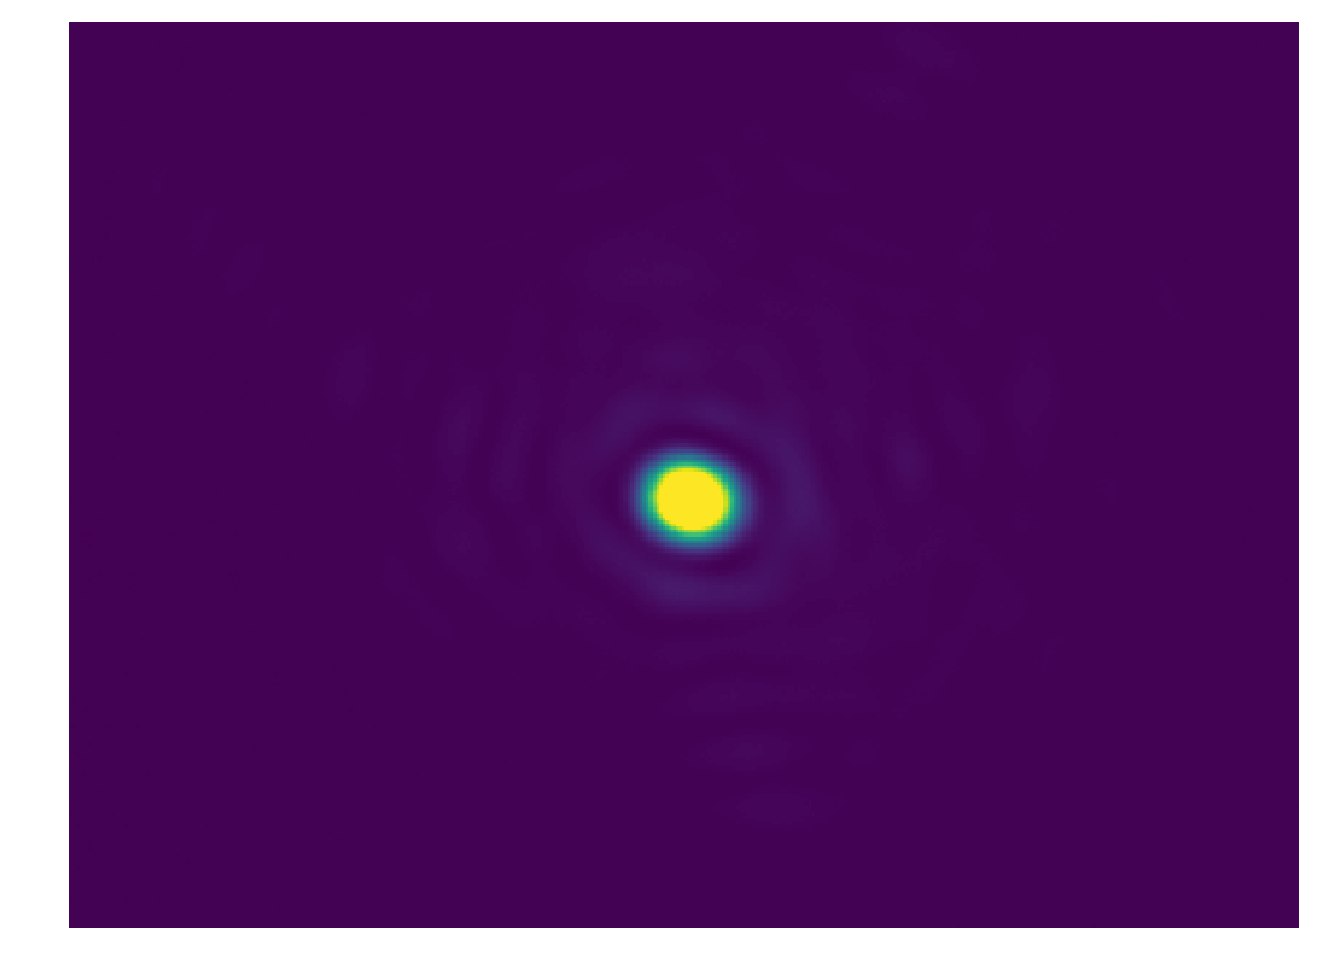
\includegraphics[width=.5\textwidth]{\figuredir{camera/profile2d.pdf}}
  \caption{Image detail from the captured beam with the \gls{ccd} camera.}
  \label{fig:beamprofile:2d}
\end{figure}

The two dimensional beam profile shows the characteristical two dimensional
gaussian distribution with diffraction rings caused by beam clipping at
finite apertures as described in \cite{Hertlein2017}.

\begin{figure}[ht]
  \centering
  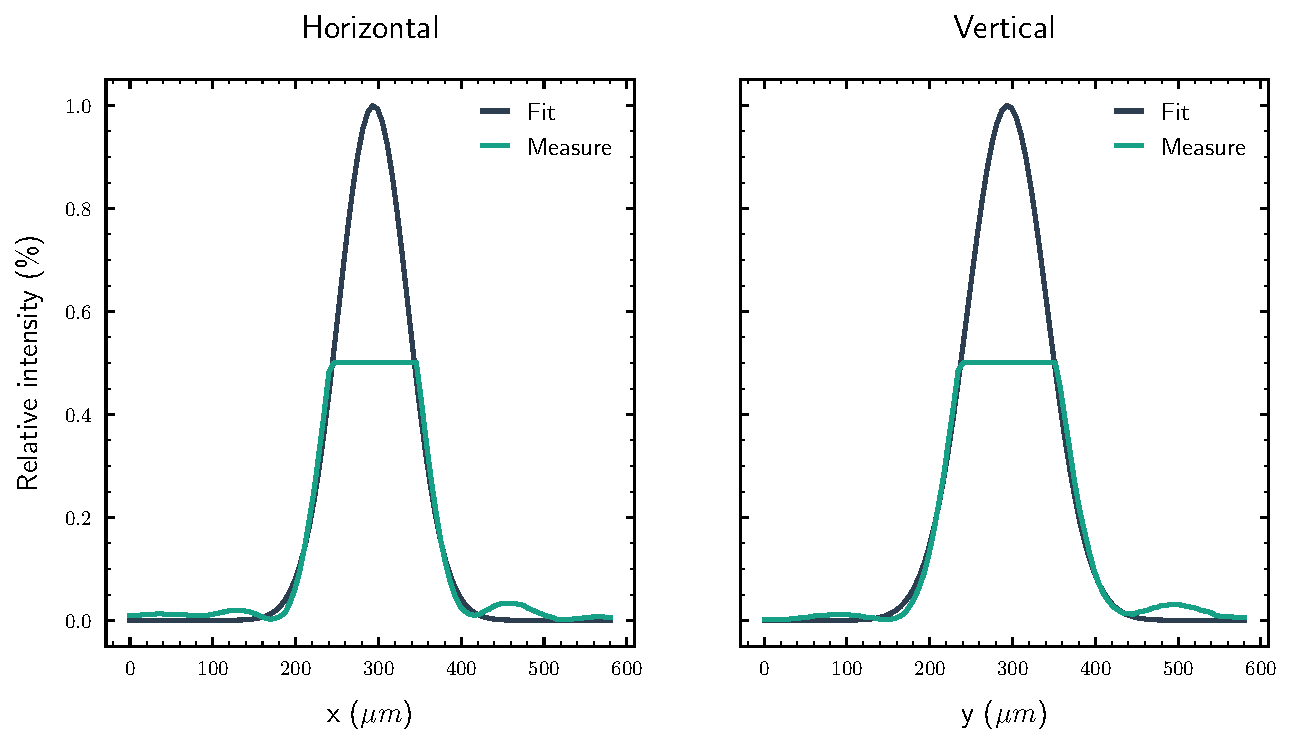
\includegraphics[width=\textwidth]{\figuredir{camera/profile1d.pdf}}
  \caption{1D horizontal and vertical profile extracted from the center of
    the image detail in \cref{fig:beamprofile:2d} with fitted gaussian curve
  and residue.}
  \label{fig:beamprofile:1d}
\end{figure}

By inspecting the one dimensional profiles with fitted gaussian and residue
we again confirm conclusions drawn in \cite{Hertlein2017}. The clipped top
of the measured intensity originates from the saturated pixels of the
\gls{ccd} camera and can be ignored. We further observe a slight assymmetry
at the diffraction rings. Overall the shown profiles can be considered to
confirm a good alignment.

\chapter{Experimental results}

% computer -> dds
%          -> scope
%          -> trigger
%          <- scope


% network analyzer (frequency dependence amplification)
% chirp signal deviation from ideal

\section{Intensity Control}
% test of long time stability

\begin{figure}[h]
  \centering
  \captionsetup{width=.8\textwidth}
  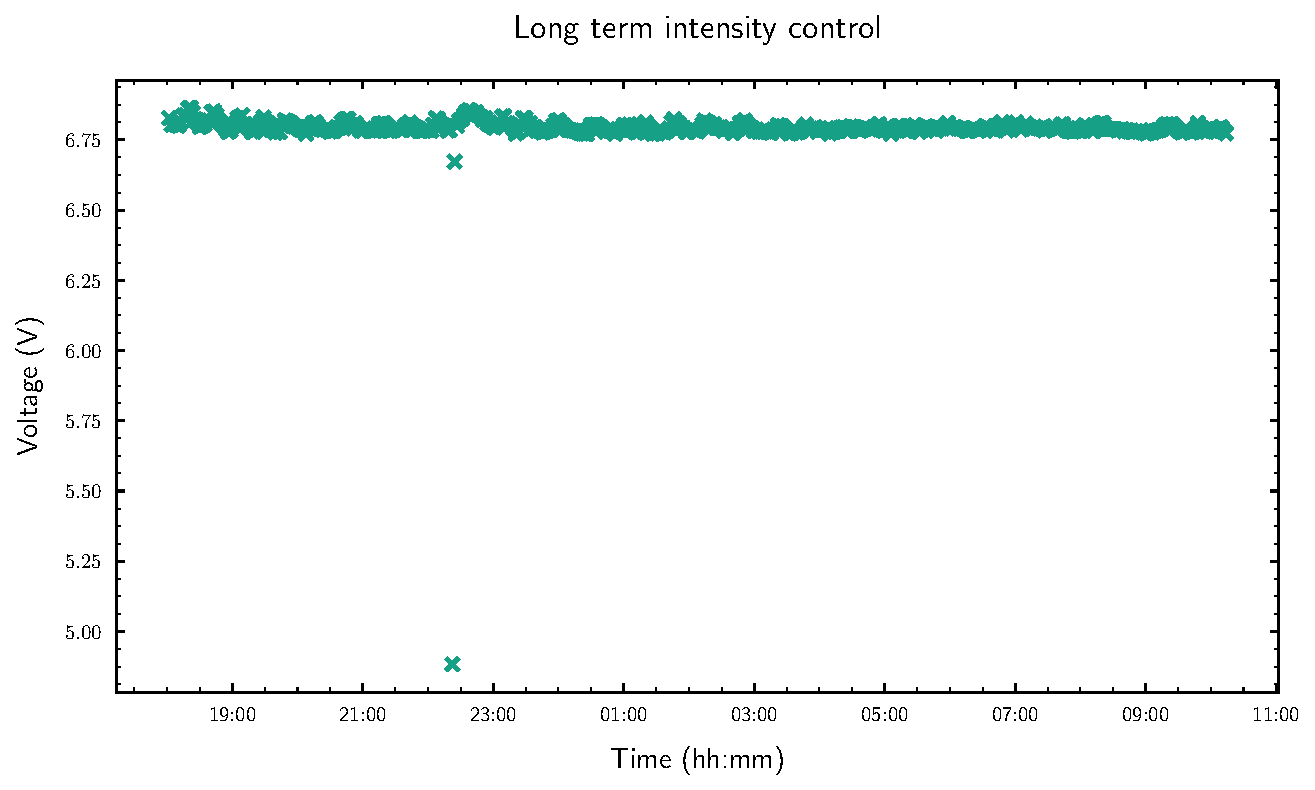
\includegraphics[width=\textwidth]{\figuredir{intensity/control-long.pdf}}
  \caption{Long measurement of the intensity without any electro-optics every
  \SI{130}{\second} for over \SI{16}{\hour} to determine the accuracy of the
  intensity controller. The outlier at around 23:00 were caused by a late
  laboratory visit.}
\end{figure}

\begin{figure}[h]
  \centering
  \captionsetup{width=.8\textwidth}
  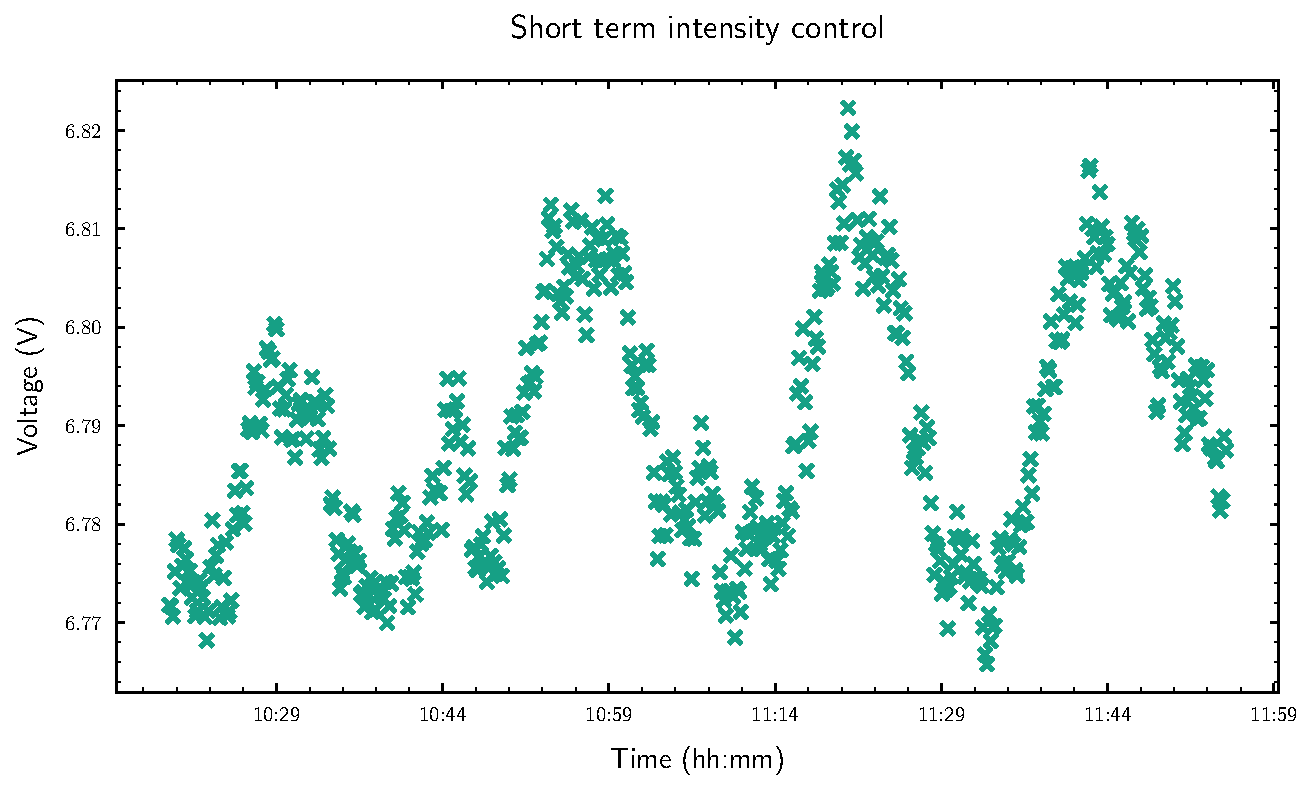
\includegraphics[width=\textwidth]{\figuredir{intensity/control-short.pdf}}
  \caption{Short measurement of the intensity without any electro-optics every
  \SI{10}{\second} for over \SI{1}{\hour} to determine the accuracy of the
  intensity controller.}
\end{figure}

\section{Synthesizer}

\begin{figure}[h]
  \centering
  \captionsetup{width=.8\textwidth}
  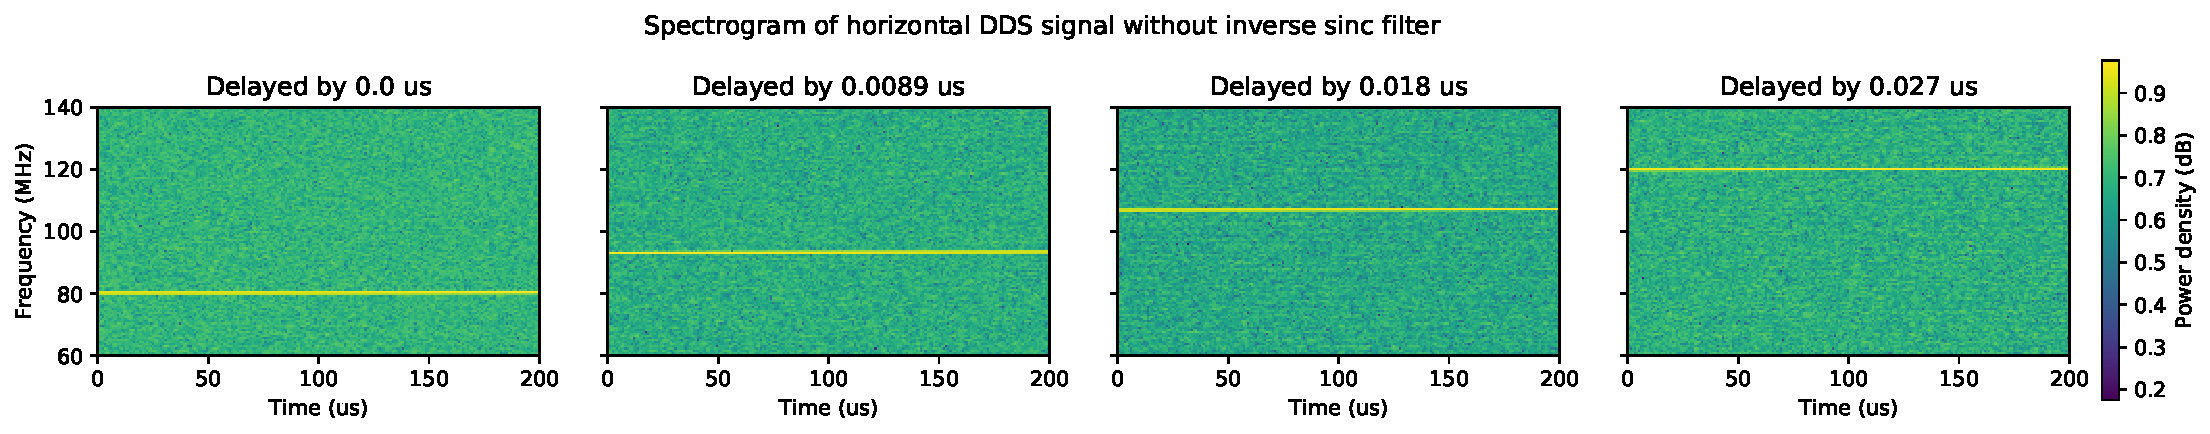
\includegraphics[width=\textwidth]{\figuredir{synthesizer/specgram.pdf}}
  \caption{Short measurement of the intensity without any electro-optics every
  \SI{10}{\second} for over \SI{1}{\hour} to determine the accuracy of the
  intensity controller.}
\end{figure}

\begin{figure}[h]
  \centering
  \captionsetup{width=.8\textwidth}
  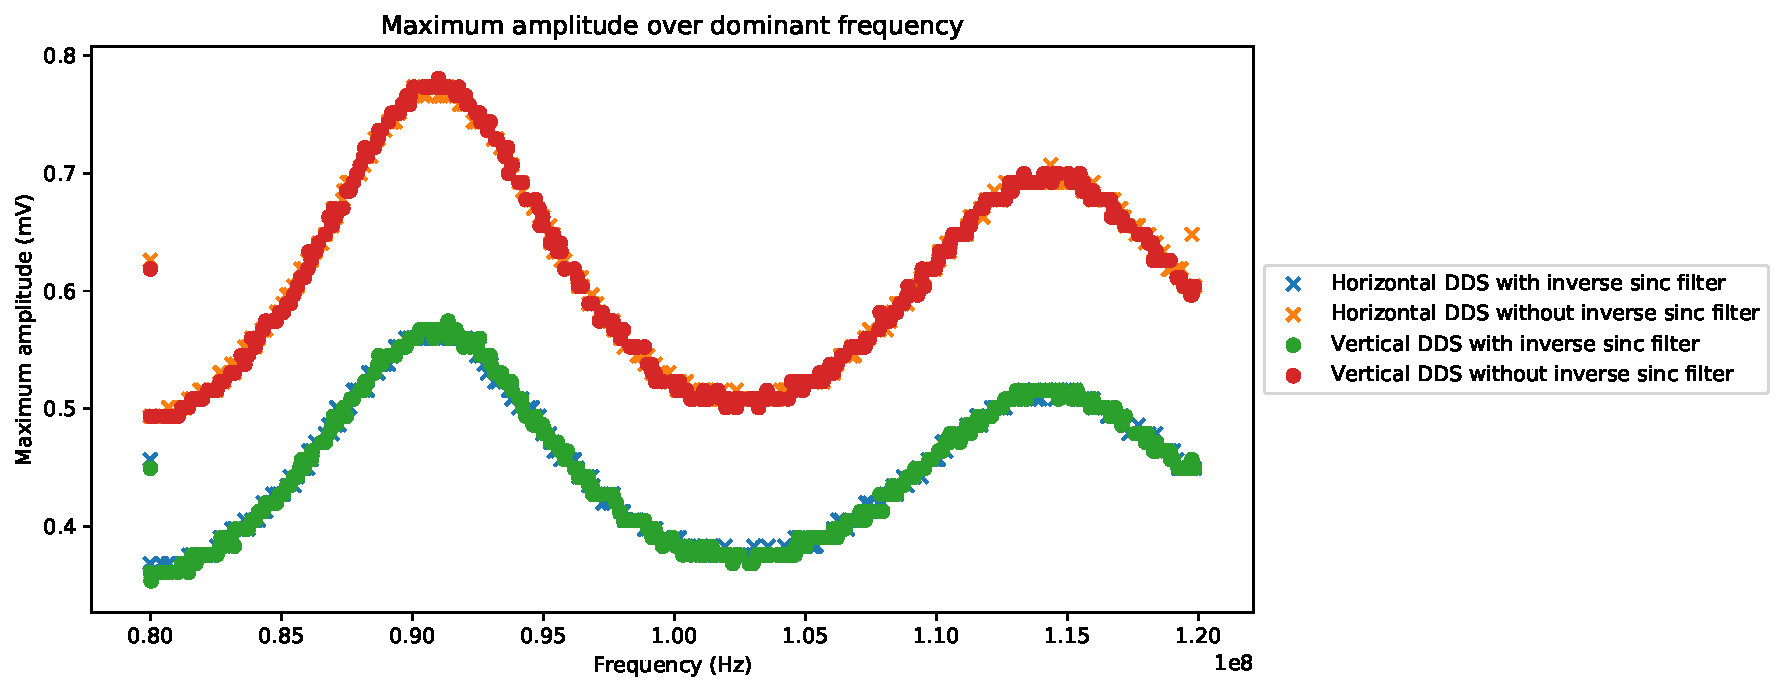
\includegraphics[width=\textwidth]{\figuredir{synthesizer/frequency.pdf}}
  \caption{Short measurement of the intensity without any electro-optics every
  \SI{10}{\second} for over \SI{1}{\hour} to determine the accuracy of the
  intensity controller.}
\end{figure}

\section{Amplifier}

\section{Acousto-optic deflector}
\subsection{Power matching}

\subsection{Intensity}
% H removed, V sweep (H in V position, vice versa)
% V removed, H sweep (V in H position, vice versa)

% H constant with V sweep
% V constant with H sweep

\chapter{Intensity Optimization}
\
% at different amplitude values
% without amplitude modulation
% with amplitude modulation

\chapter{Conclusion}

\section{Summary}

\section{Future Outlook}

\section{Further Applications}


\printglossaries
\listoffigures
\listoftables
\listoflistings
\printbibliography

\appendix
\chapter{Electronics}

\section{Trigger Hub}
\label{app:electronics:trigger_hub}

The trigger hub is driven by a \SI{3.3}{\volt} input signal and a
\SI{5}{\volt} voltage source. The input signal is amplified to drive four
\gls{ttl} inputs through use of the \gls{sn74128} \cite{SN74128} line driver.
Furthermore the hub is designed to be mounted on the \gls{bbb} which itself
provides the trigger network interface.

\begin{figure}[h]
  \centering
  \captionsetup{width=.8\textwidth}
  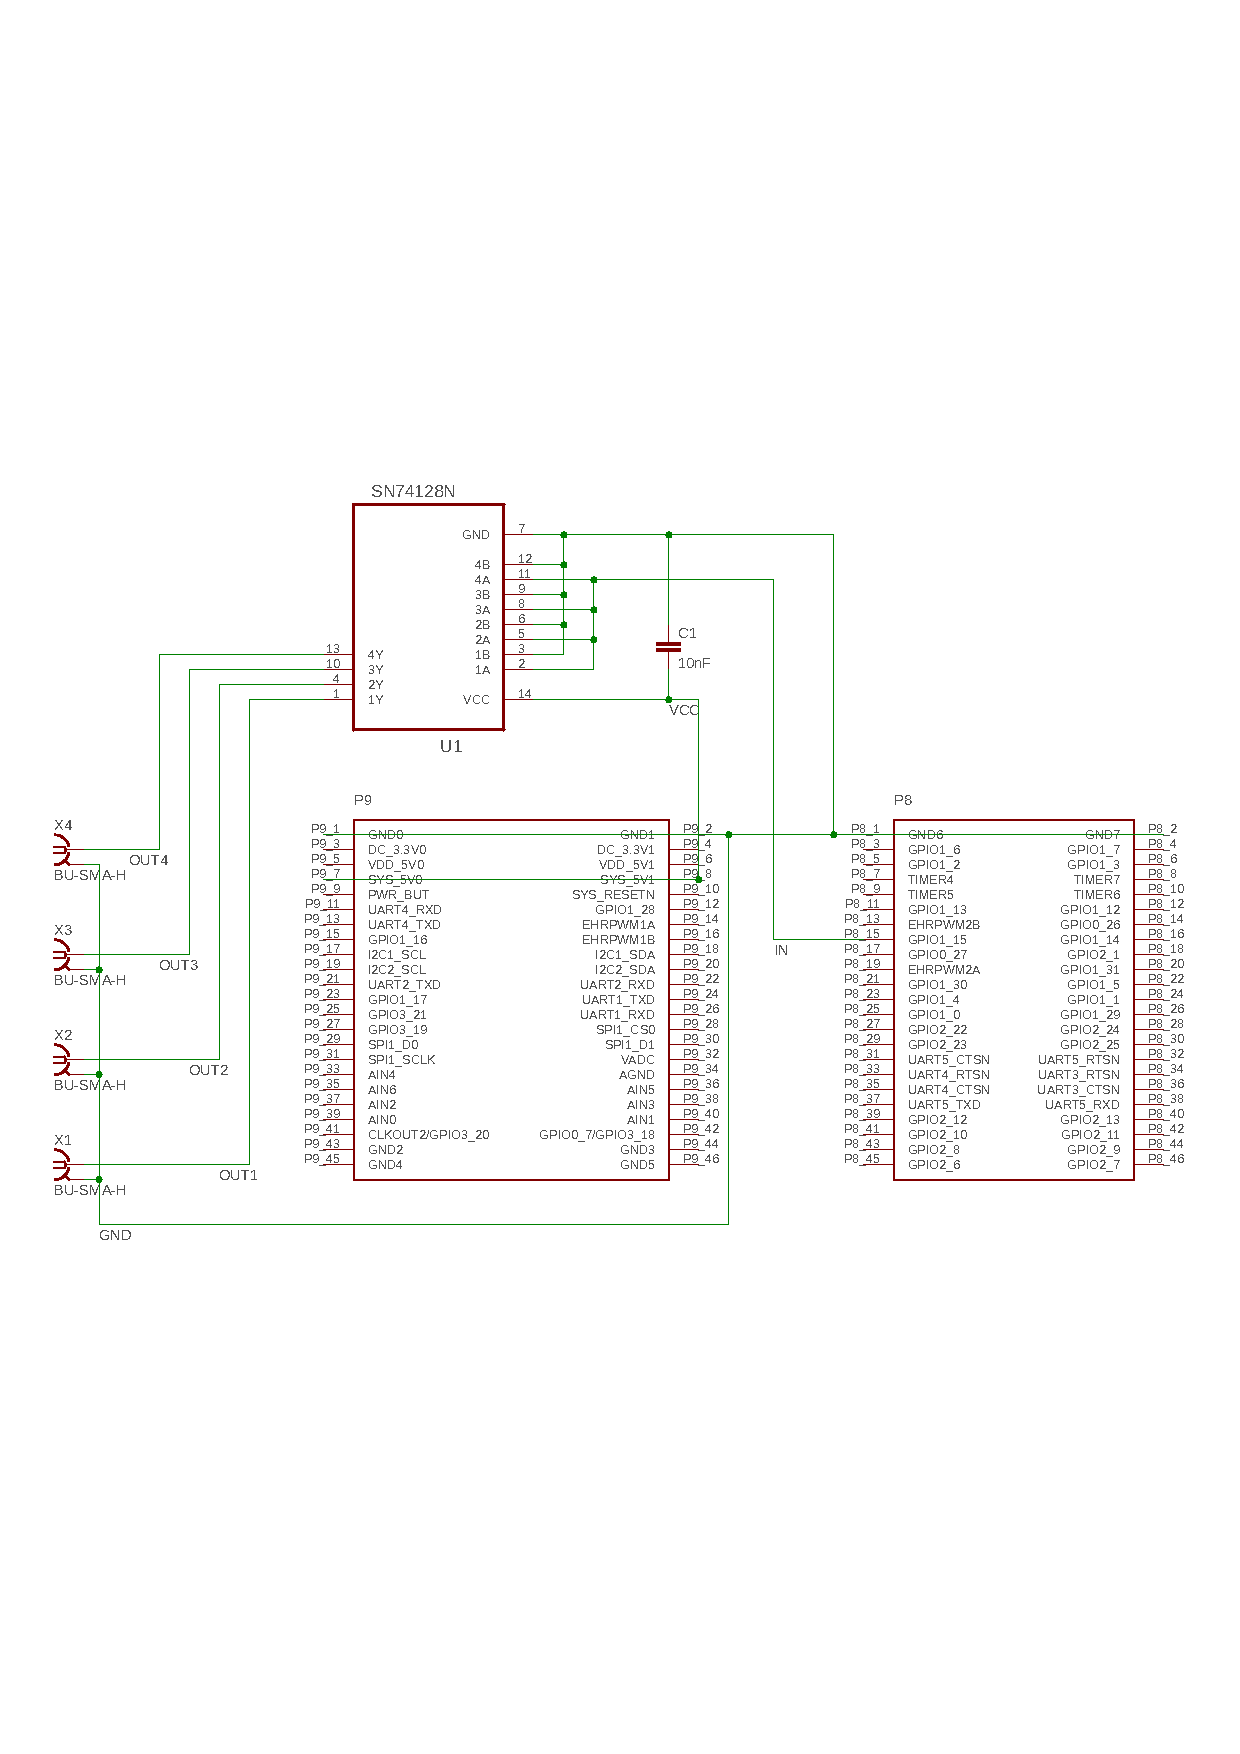
\includegraphics[width=\textwidth]{images/circuits/line-driver/schematic.pdf}
  \caption{Elecronic circuit schematics of the trigger hub. The
    \SI{3.3}{\volt} input signal is amplified by the \gls{sn74128} line
    driver and outputed to four \gls{sma} connectors.}
\end{figure}

The \gls{sn74128} exposes four independent outputs $Y$, each is driven by a
two-input ($A$ and $B$) with NOR ($\overline{A+B}=Y$) logic. As our objective
is to forward rising edge trigger signals we pulled all four $B$ to low by
connecting them with \gls{gnd}. The four $A$ where connected together with
the input signal. The input signal has to transition from $1$ to $0$ in order
to signal a rising edge trigger signal.

\begin{listing}[h]
  \inputminted[xleftmargin=.2\linewidth]{javascript}{scripts/trigger.js}
  \captionsetup{width=.6\linewidth}
  \caption{\gls{bbb} script that starts a \gls{http} server to listen for
requests on which to trigger a rising edge signal. On execution it pulls the
signal \gls{gpio} to high. The request callback then pulls the \gls{gpio} to
low for one \SI{1}{\milli\second}.}
\end{listing}

Using the \gls{bbb} makes it easy to write scripts that communicate with
other devices over the \gls{lan}. We used the bonescript library to access
the \gls{gpio} interface as it is pre-installed on the \gls{bbb}.

\begin{figure}[h]
  \centering
  \begin{minipage}{.40\textwidth}
    \centering
    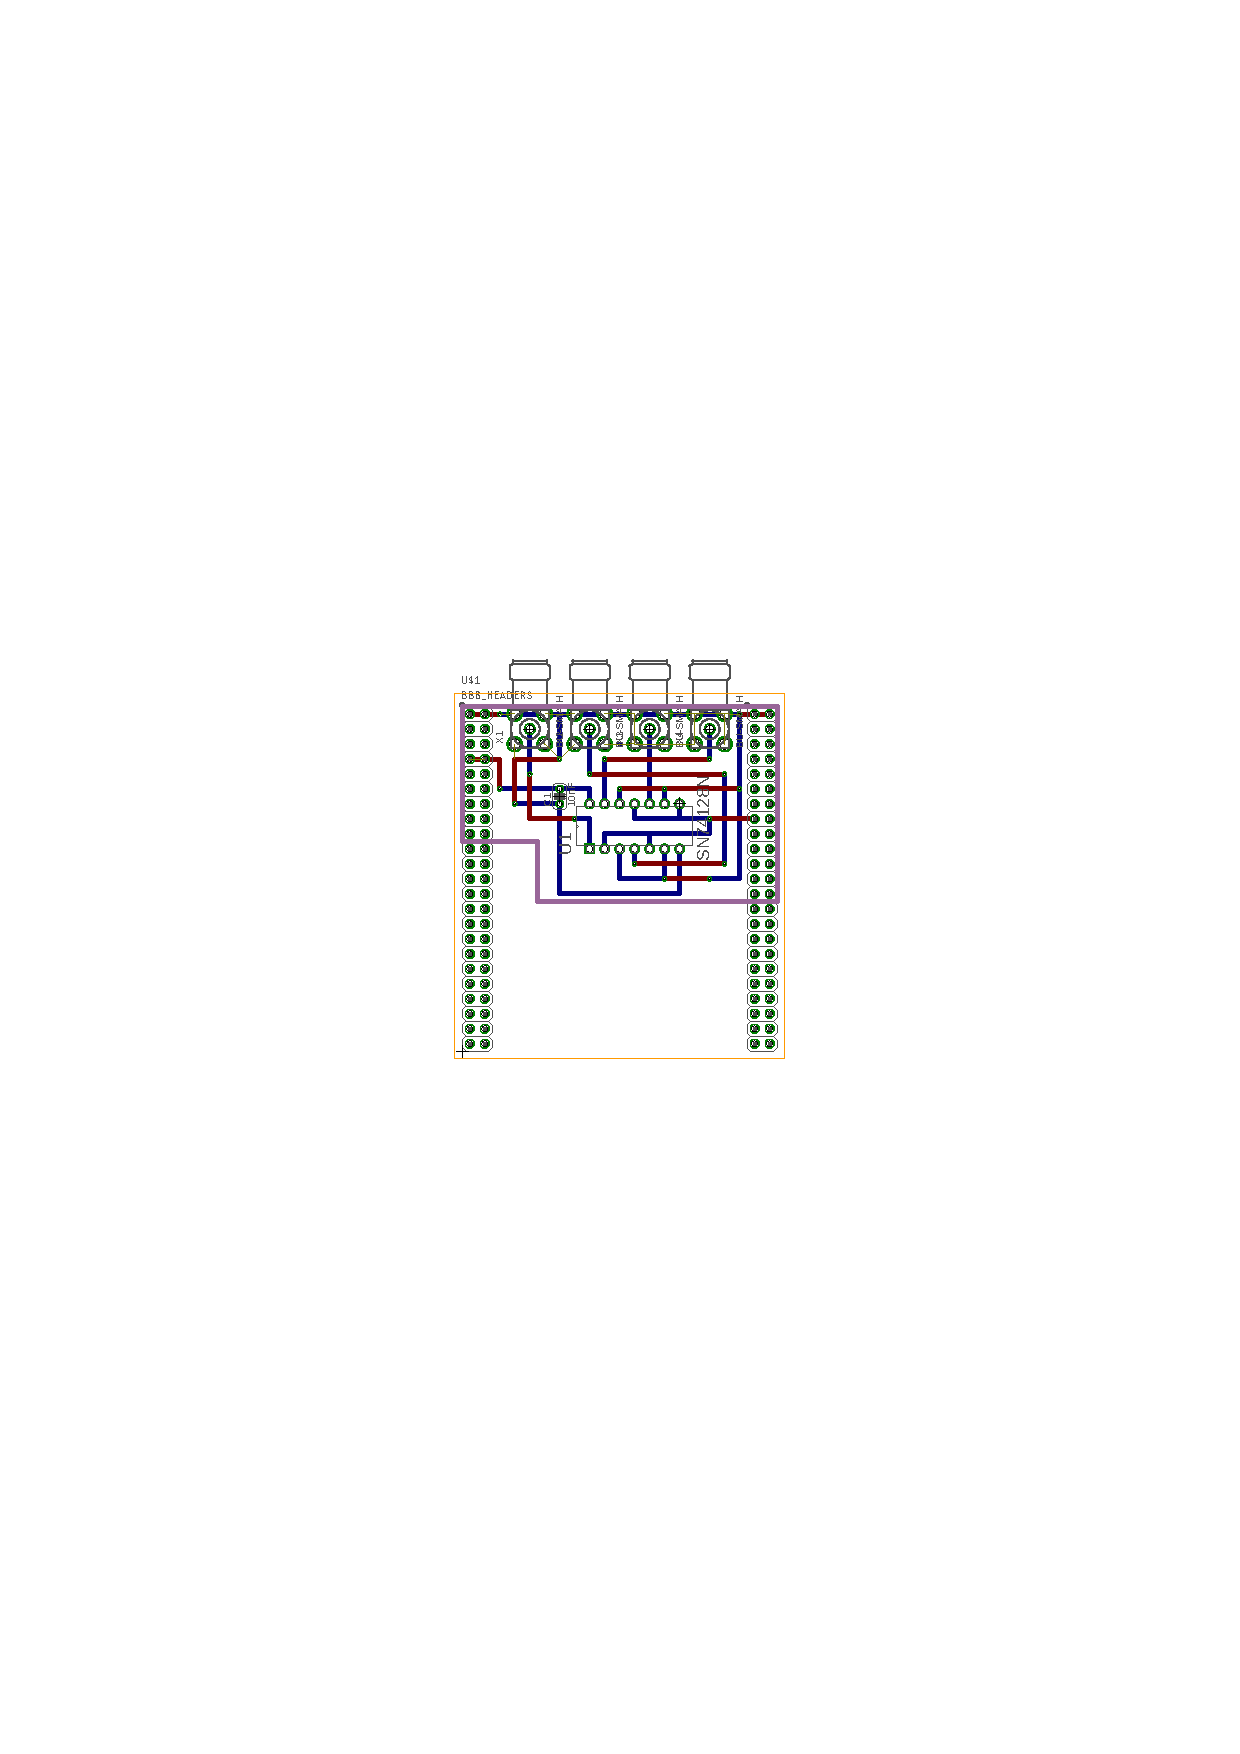
\includegraphics[width=\linewidth]{images/circuits/line-driver/layout.pdf}
    \captionsetup{width=\linewidth}
    \caption{Board layout of the trigger hub. The source amplifier is designed
to fit on top of the \gls{bbb} expansion headers.}
  \end{minipage}
  \begin{minipage}{.50\textwidth}
    \centering
    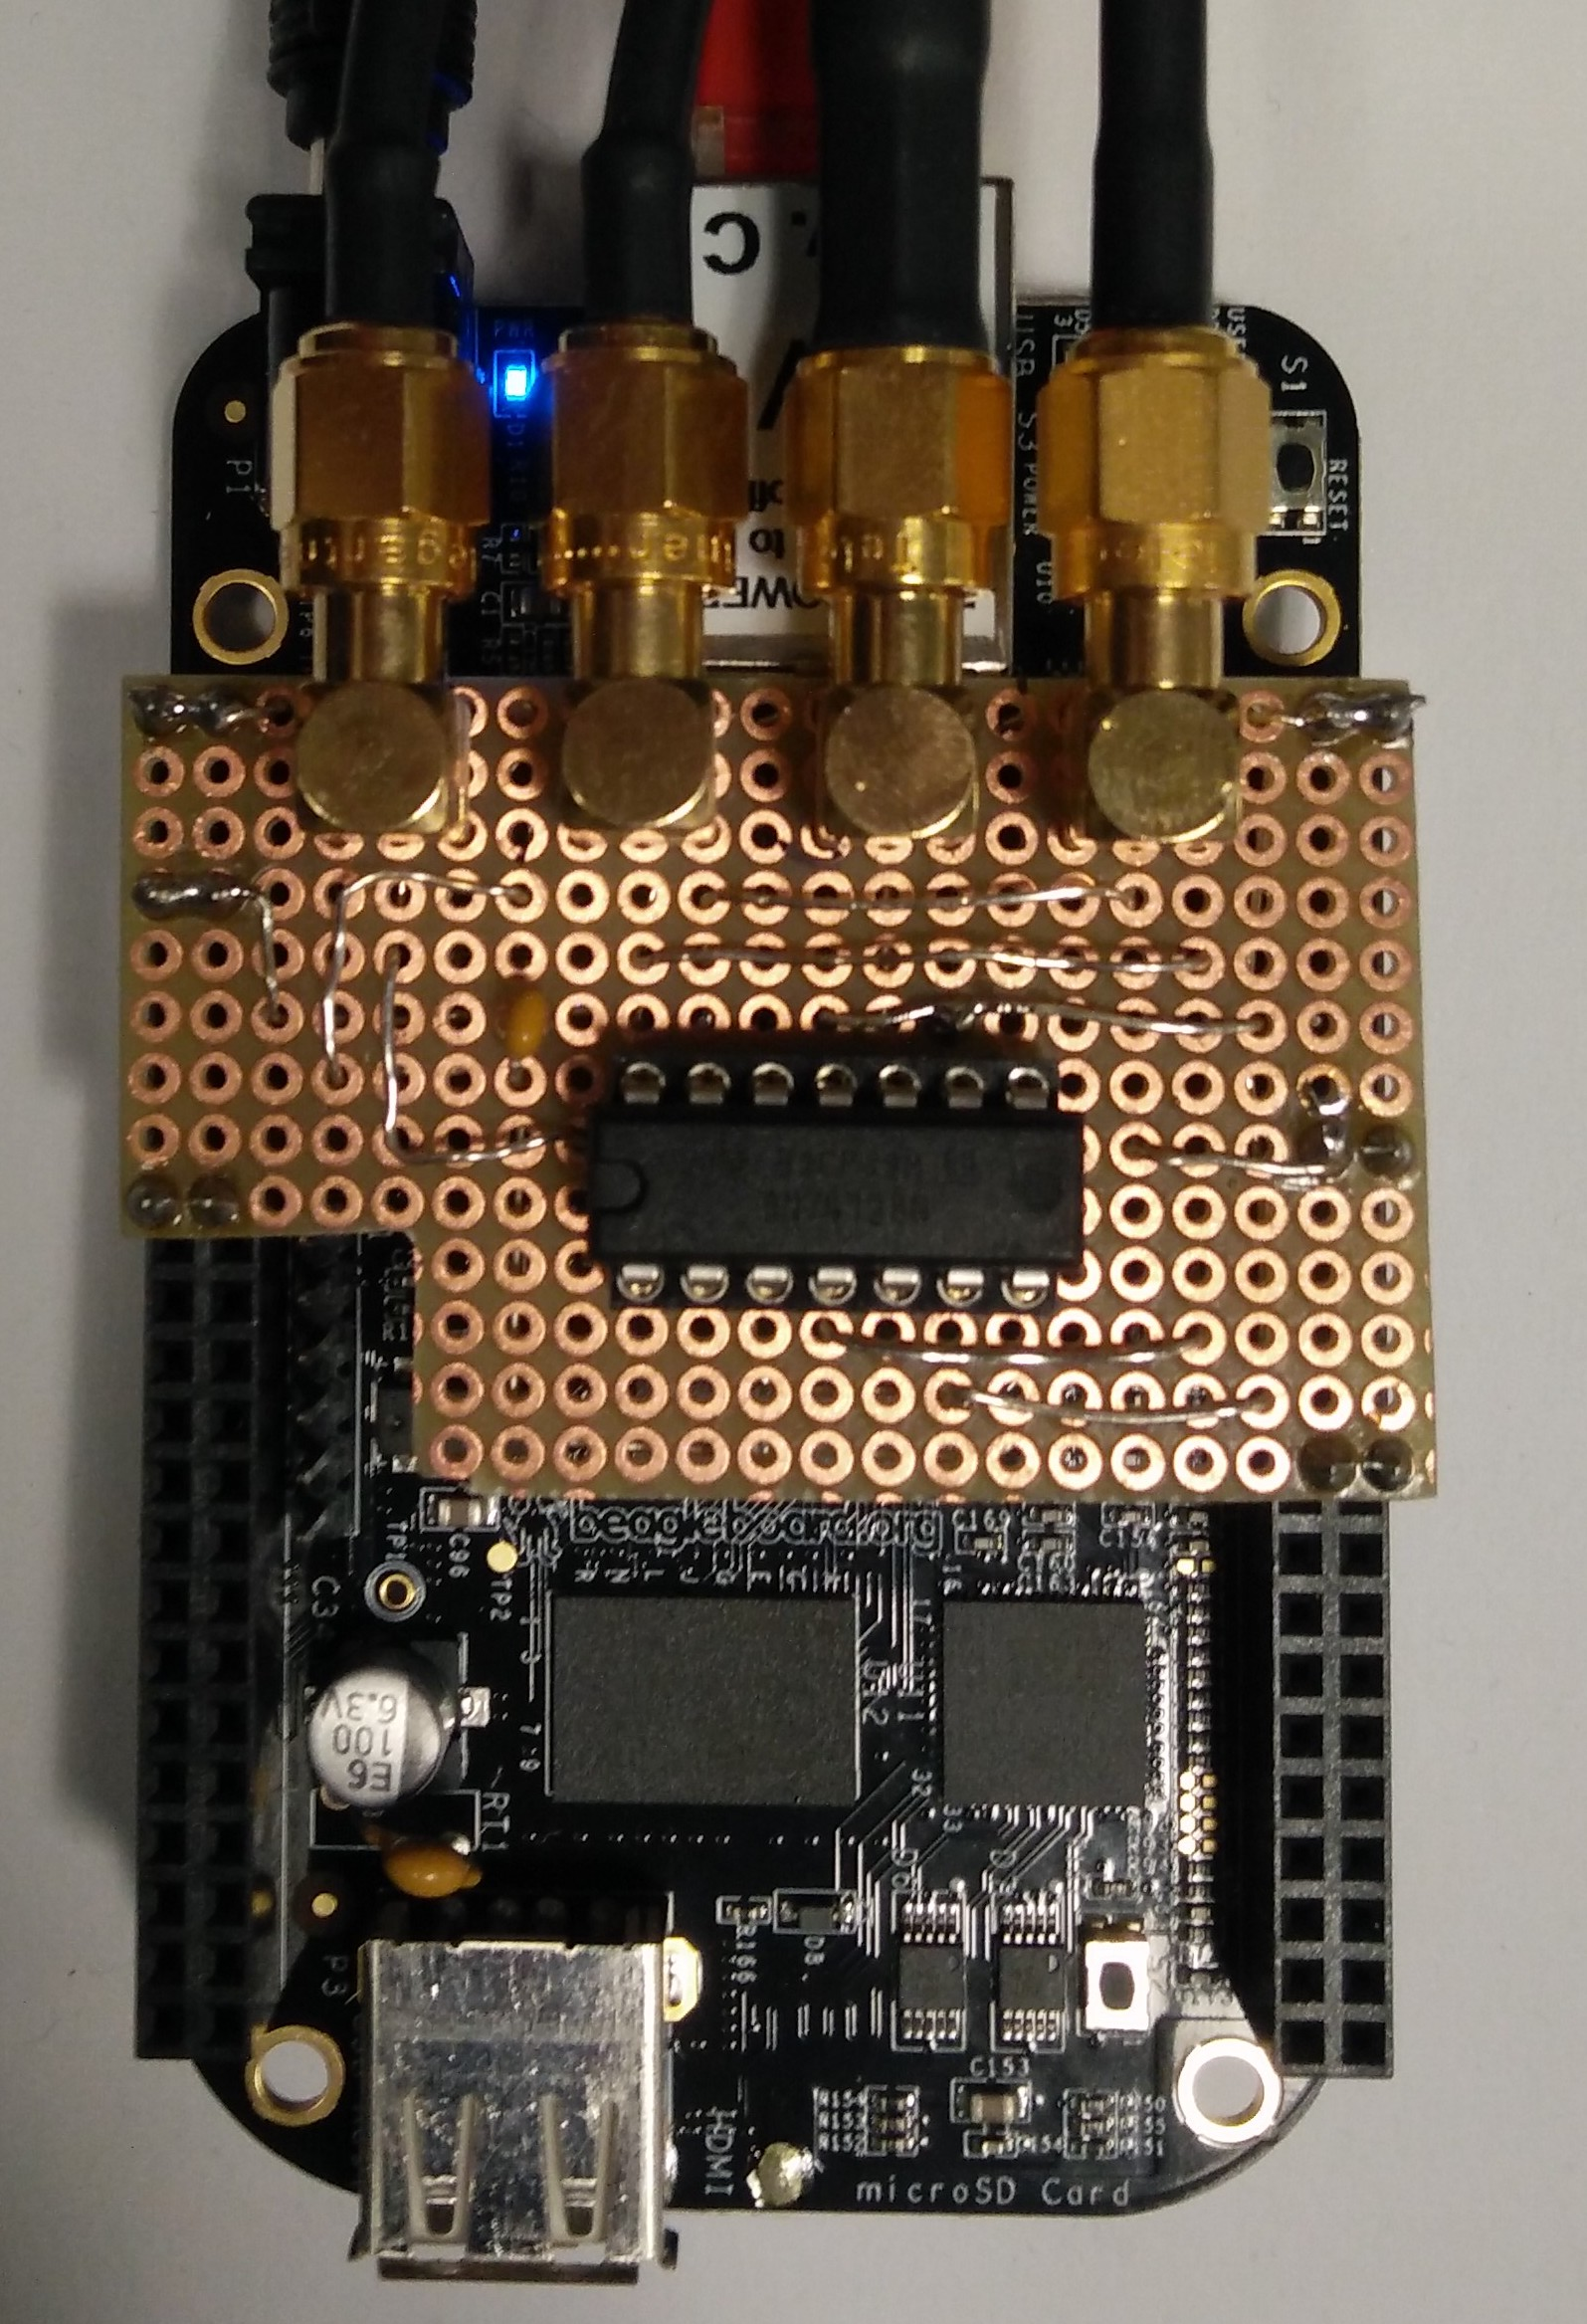
\includegraphics[width=.6\linewidth]{images/circuits/line-driver/board.jpg}
    \captionsetup{width=.8\linewidth}
    \caption{Picture of the trigger hub on the \gls{bbb}. The \gls{bbb} is
connected with the \gls{lan} via cable. The trigger hub forwards the signal
to the oscilloscope, the camera and the two \gls{dds}.}
  \end{minipage}
\end{figure}

\chapter{Calibration}

Alterations of the laboratory environment combined with the exchange of
components from the original setup made it advisable to recalibrate the setup.
In this chapter we want to document the steps necessary for calibration for
successive experiments.

\section{Fiber Coupling}

The visually shielded section of the setup used to reduce the output power
of the laser source is optically paired with the open section for beam
deflection via a \gls{smf} that only permits two orthogonal polarization and
a single gaussian mode. Through tuning the polarisator inside the power
reduction section we can try to match one of the orthogonal polarization
modes supported by the \gls{smf}. Polarization discrepancies induce the
polarization inside the \gls{smf} to oscillate on environmental changes like
temperature or vibration. Henceforth it is key to couple polarization modes
in order to ensure a stable operation.

The following receipt has proven to be successful to find an approximate
polarization match between the laser beam and the \gls{smf}. In addition
to the setup described in \cref{sec:powerbox} and \cref{sec:deflection}
an oscilloscope and a hot air gun are highly recommended.

\begin{enumerate}
  \item Connect the photodiode to the oscilloscope and use a coarse time
    scale of i.e. \SI{2}{\second}.
  \item Apply safety measures i.e. put on appropiete laser safety glasses and
    inform present personal of the imminent danger.
  \item Open the cover of the power reduction setup.
  \item Apply heat to the \gls{smf} through the hot air gun, alternatively
    you can try to move the fiber.
  \item The photodiode signal should start to oscillate. Tune the polarizor
    inside the power reduction subject to minimizing the oscillation.
\end{enumerate}

The oscillations occur as the polarization circulates inside the fiber and
will stop at some point. In this case yu should remove the heat or mechanical 
stress on the fiber and wait some time before you can reapply with the initial
response.

\section{Beam Alignment}

As is well known, beams that pass off-centered through spherical lenses
experience optical aberrations. Additionally we found that uncentered beams
may cause further optical defects from reflections at boundaries. Both effects
should be avoided as far as possible by adjusting positions and mirror angles.

As auxilliaries we recommend a pair of iris diaphragms that are mountable to
the lens mounts and a screen i.e. a white sheet of hard paper. With the iris
diaphragms we can easily find a center reference point visually by inspecting
the symmetry of the iris illumination at different pinhole diameters. Exact
steps are summarized in the below receipt. We refer to the optics as annotated
in \cref{fig:deflection}.

\begin{enumerate}
  \item Place screen in front of L2 and adjust screws on fiber coupler subject
    to a clean beam profile on the screen of the (1,1) diffraction order of
    the \gls{aom}s.
  \item Apply one iris to L2 and find center frequency of the \gls{aom}s.
  \item Mount irises on L3 and L4. Mount mirror pair M1, M2 to direct beam
    through both pinholes.
  \item Place auxilliary lens with mounted iris between L7 and M3 and adjust
    second objective pair L6, L7.
  \item Mount iris on L8 and place auxilliary lens with mounted iris in front
    of BS3. Align the mirror pair M3 and M4 to reflect the beam through both
    irises.
  \item Adjust the objective pair distance until you see an output similar to
    XY on the \gls{ccd} camera.
\end{enumerate}

The alignment of a mirror pair can be simplified by using the below algorithm:

\begin{enumerate}
  \item Select axis to align.
  \item Align the beam on the outside lens by tuning the inner mirror.
  \item Align the beam on the inner lens by tuning the outside mirror.
  \item Repeat steps 2 and 3 until beam is aligned on both lenses. Proceed
    with other axis.
\end{enumerate}

\section{Camera Focus}

Finally we had to reposition the camera to focus the incoming beam correctly
in order to register the beam profile as would be seen later by the atoms.
To find the precise focus position we followed the procedure described in
\cite{Hertlein2017} that consits of extracting the camera rail with its lens
and focusing it on a far distant object.

\begin{figure}[ht]
  \centering
  \includegraphics[width=\textwidth]{\builddir{focus.pdf}}
  \caption{Camera focused on far distant object. In this case a window from the
  building accross the courtyard.}
\end{figure}

\section{Beam Profile}

% Image from CCD camera with gaussian fit


\end{document}
